%\documentclass[a4paper,12pt]{report}
\documentclass[a4paper,12pt]{extreport}


%%% Поля и разметка страницы %%%
\usepackage{lscape}	    % Для включения альбомных страниц
\usepackage{geometry}	% Для последующего задания полей
%\usepackage{subfigure}  % Для создания рисунков с несколькими панелями

%%% Кодировки и шрифты %%%
\usepackage{cmap}			% Улучшенный поиск русских слов в полученном pdf-файле
\usepackage[T2A]{fontenc}		% Поддержка русских букв
\usepackage[utf8]{inputenc}		% Кодировка utf8
\usepackage[english, russian]{babel}	% Языки: русский, английский
%\usepackage{pscyr}			% Красивые русские шрифты
\usepackage{braket}

%%% Математические пакеты %%%
\usepackage{amsthm,amsfonts,amsmath,amssymb,amscd} % Математические дополнения от AMS

%%% Оформление абзацев %%%
\usepackage{indentfirst} % Красная строка

%%% Цвета %%%
\usepackage[usenames]{color}
\usepackage{color}
\usepackage{colortbl}

%%% Таблицы %%%                        
%\usepackage{longtable}			% Длинные таблицы
%\usepackage{multirow,makecell,array}	% Улучшенное форматирование таблиц

%%% Общее форматирование
\usepackage[singlelinecheck=off]{caption}	% Многострочные подписи
%\usepackage{soul}					% Поддержка переносоустойчивых подчёркиваний и зачёркиваний

%%% Библиография %%%
\usepackage[numbers]{natbib}
%\usepackage{cite} % Красивые ссылки на литературу
%\usepackage{csquotes}
%\usepackage[autolang=other,       
%            bibencoding=utf8,
%            sorting=none, % Name,Title,Year или sorting=none.
%            maxbibnames=3, % Максимальное число авторов в списке литературы.
%            minbibnames=2, % Число авторов, отображаемое при сокращении.
%            style=gost-numeric,
%            backend=biber]{biblatex}


\usepackage{placeins}

%%% Гиперссылки %%%
\usepackage[linktocpage=true,plainpages=false,pdfpagelabels=false,unicode=true]{hyperref}

%%% Изображения %%%
\usepackage{graphicx} % Подключаем пакет работы с графикой
%\usepackage{epstopdf}

%%% Оглавление %%%
\usepackage{tocloft}

\usepackage{titlesec}

%\usepackage{minted} %консольные комманды
\usepackage{listings}
\usepackage{tabularx} %растягивание колонок и перенос текста
\usepackage{xtab} %многостраничные таблицы
		% Подключаемые пакеты
%%% Макет страницы %%%
\geometry{a4paper,top=2cm,bottom=2cm,left=2cm,right=2cm}

\titleformat{\chapter}[display]
  {\normalfont\Large\filcenter\bfseries}{\chaptertitlename\ \thechapter}{20pt}{\LARGE}
\titlespacing*{\chapter}
  {0pt}{30pt}{20pt}

% см. http://tex.stackexchange.com/questions/134031/how-to-adjust-the-size-and-placement-of-chapter-heading-in-report-class
% и http://tex.stackexchange.com/questions/59726/change-size-of-section-subsection-subsubsection-paragraph-and-subparagraph-ti

%%% Кодировки и шрифты %%%
%\renewcommand{\rmdefault}{ftm} % Включаем Times New Roman

%%% Выравнивание и переносы %%%
\sloppy					% Избавляемся от переполнений
\clubpenalty=10000		% Запрещаем разрыв страницы после первой строки абзаца
\widowpenalty=10000		% Запрещаем разрыв страницы после последней строки абзаца
\linespread{1.3}

%%% Библиография %%%
\makeatletter
\bibliographystyle{ugost2008ns_v1.bst}	% Оформляем библиографию в соответствии с ГОСТ 7.0.5
%\bibliographystyle{utf8gost705u}
%\bibliographystyle{ugost2008}
\renewcommand{\@biblabel}[1]{#1.}	% Заменяем библиографию с квадратных скобок на точку:
\makeatother

%%% Изображения %%%
\graphicspath{{img_part1/}{img_part2/}{img_part3/}{img_part4/}{img_part5/}} % Пути к изображениям

%%% Цвета гиперссылок %%%
\definecolor{linkcolor}{rgb}{0.9,0,0}
\definecolor{citecolor}{rgb}{0,0,1}
\definecolor{urlcolor}{rgb}{0,0,1}
\hypersetup{
    colorlinks, linkcolor={linkcolor},
    citecolor={citecolor}, urlcolor={urlcolor}
}

%%% Оглавление %%%
\renewcommand{\cftchapdotsep}{\cftdotsep}


\newcommand{\kws}{\textit{KW}\ }
\newcommand{\rmn}[1]{{\mathrm{#1}}}
\newcommand\fdg{\mbox{$.\!\!^\circ$}}%
\newcommand\farcm{\mbox{$.\mkern-4mu^\prime$}}%
\newcommand\farcs{\mbox{$.\!\!^{\prime\prime}$}}%
\newcommand\nodata{ ~$\cdots$~ }%

			% Пользовательские стили

% journals

\def\apj{ApJ}
\def\apjl{ApJ Lett.}
\def\mnras{MNRAS}
\def\nat{Nature}
\def\physrevB{Phys. Rev. B}
\def\prd{Phys. Rev. D}
\def\prl{Phys. Rev. Lett.}
\def\pre{Phys. Rev. E}
\def\araa{Ann. Rev. Astron. Astrophys.}                % "Ann. Rev. Astron. Astrophys."
\def\aap{Astron. Astrophys.}                  % "Astron. Astrophys."
\def\aaps{Astron. Astrophys. Suppl. Ser.}                 % "Astron. Astrophys. Suppl. Ser."
\def\aj{Astron. J.}                      % "Astron. J."
\def\apjs{Astrophys. J. Suppl. Ser.}                  % "Astrophys. J. Suppl. Ser."
\def\pasp{Publ. Astron. Soc. Pac.}                  % "Publ. Astron. Soc. Pac."
\def\apjl{ApJ Lett.}                   % letter at ApJ
\def\pasj{PASJ}
\def\apss{Astroph. Space Sci.}
\def\aplett{Astroph. Lett.}
\def\ssr{Space Sci. Rev.}
\def\jcap{J. Cosmol. Astropart. Phys.}
\def\apspr{Sov. Sci. Rev. Sect. E}
\def\nar{New Astron. Rev.}
\def\aapr{ Astron. Astrophys. Rev.}

\begin{document}
	
	%%% Переопределение именований %%%
\renewcommand{\abstractname}{Abstract}
\renewcommand{\alsoname}{see also}
\renewcommand{\appendixname}{Appendix}
\renewcommand{\bibname}{References}
\renewcommand{\ccname}{Source}
\renewcommand{\chaptername}{Chapter}
\renewcommand{\contentsname}{Contents}
\renewcommand{\enclname}{include}
\renewcommand{\figurename}{Figure}
\renewcommand{\indexname}{Index}
\renewcommand{\listfigurename}{Figures list}
\renewcommand{\listtablename}{Tables list}
\renewcommand{\pagename}{page}
\renewcommand{\partname}{Part}
\renewcommand{\refname}{References}
\renewcommand{\seename}{see}
\renewcommand{\tablename}{Table}
			% Переопределение именований
	
	\thispagestyle{empty}



\begin{center}
{
Ioffe Institute of Russian Academy of Science\\
}
\end{center}

\begin{figure}
	\centering
	
\includegraphics[width=5.5 cm]{./fig/ioffe.png} 
\end{figure}



\vspace{5mm}
\begin{center}
{\bf \Huge FAINA
\par}
\vspace{10mm}
%Astrophysical code for modeling radiation sources 
Numerical code for modeling electromagnetic radiationfrom astrophysical sources

\vspace{10mm}
%User's guide
{\bf \large User's guide \par}
\end{center}




\vspace{120mm}
\begin{center}
{Saint-Petersburg~--- 2023}
\end{center}

\newpage			% Титульный лист
	\tableofcontents
\clearpage
		% Оглавление
	\chapter*{Introduction}		
\addcontentsline{toc}{chapter}{Introduction}	%добавляем в оглавление			
FAINA - is a numerical code for modeling different types of electromagnetic radiation of astrophysical source. It is written in C++ and supports parallel computations using openmp method. FAINA allows to model observable fluxes from sources with different parameters and geometries vai different emission mechanisms, and also to optimize source parameters to fit observational data.

\section*{Installation}
\addcontentsline{toc}{section}{Installation}
Current version of the code is available on github https://github.com/VadimRomansky/Faina. FAINA is distributed freely under the MIT public license. Download the archive with code and extract it into preferred root directory.

\subsection*{Windows}
\addcontentsline{toc}{subsection}{Windows}
With Windows OS it is recomended to use Microsoft Visual Studio and open solution Faina.sin with it. Operability was examined for Windows 10 and Visual Studio 2022 version.

\subsection*{Unix}
\addcontentsline{toc}{subsection}{Unix}
There are two possible ways to run FAINA on Unix. We recommend to use IDE QtCreator and open  with it file Faina.pro located in the rrot directory.

Other way is to use FAINA from terminal. To compile and run it you can use following commands

\begin{lstlisting}[language=bash]
	$ make
	$ ./Faina
\end{lstlisting}

Operability was examined for Ubuntu 22.04.

\section*{Runnng simple problem}\label{running}
\addcontentsline{toc}{section}{Runnng simple problem}

Let see a simple example of solving radiation problem with faina. You can find in the function evaluateSimpleSynchrotron in the file /Src/examples.cpp. Synchrotron radiation from homogenous source with   the shape of cylinder with axis along line of sight and with powerlaw electron distribution is evaluated in this example. But it demonstrates a general approach to evaluation of radiation with FAINA code.

Let define values of magnetic field and electron number density in the source (code uses CGS units).

\begin{lstlisting}[language=c++]
	double B = 1.0;
	double electronConcentration = 1.0;
\end{lstlisting}

Then you need to create distribution of emitting electrons. There are a different type of particle distribution implemented in the code, let use isotropic powerlaw distribution for this example. You should call the constructor of MassiveParticlePowerLawDistribution with following parameters - mass of emitting particles (electrons in this case), powerlaw index of distribution, which is defined as positive number $p$ in $F(E) ~ 1/E^p$, starting energy of powerlaw distribution, and electrons number density. 

\begin{lstlisting}[language=c++]
	MassiveParticleDistribution* distribution =
	new MassiveParticlePowerLawDistribution(
	massElectron, 3.0, me_c2, electronConcentration);
\end{lstlisting}

After that you should create a radiation source, for example it would be homogenous flat disk with axis along line of sight. You should call the constructor of SimpleFlatSource with following parameters: electrons distribution, magnetic field, sinus of it's inclination angle to the line of sight, radous of cylinder, it's hight and distance to the observer.

\begin{lstlisting}[language=c++]
	RadiationSource* source = new SimpleFlatSource(
	distribution, B, 1.0, parsec, parsec, 1000 * parsec);
\end{lstlisting}

And the last thing you need is an radiation evaluator. They are different for every specific type of radiation. Here we create a SybchrotronEvaluator with following parameters: number of grid points for integration electron distribution function over energy, lower and upper limits of electron energy that will be taken into account and boolean parameter determining include synchrotron self absorption or not.

\begin{lstlisting}[language=c++]
	RadiationEvaluator* evaluator = new 
	SynchrotronEvaluator(1000, me_c2, 1000 * me_c2, true);
\end{lstlisting}

Synchrotron approximation is valid only for frequencies of radiation much greater than cyclotron frequency, so let evaluate it

\begin{lstlisting}[language=c++]
	double cyclOmega = 
	electron_charge * B / (massElectron * speed_of_light);
\end{lstlisting}

Now you can evaluate spectrum of synchrotron radiation. Radiation evaluator has a method writeFluxFromSourceToFile which allows to calculate flux energy density and write it into the file in units energy vs power per energy per area, or $\rm erg$ vs $\rm sm^-2 s^-1$. This method takes following input parametes: output file name which will be created or rewritten, lower and upper limits of energy range and number of grid points, which will be distributed logarithmically in the range. If you need other units you should use method evaluateFluxFromSource which provides a flux energy density at given energy and rewrite output.

\begin{lstlisting}[language=c++]
	evaluator->writeFluxFromSourceToFile("out.dat",source, 
	10*hplank*cyclOmega, 1E5*hplank*cyclOmega, 1000);
\end{lstlisting}


Evaluated spectrum of flux energy density from this source is shown in \ref{example0}. Examples of plotting scripts you can find in Figure directory pyFAINA.
\begin{figure}
	\centering
	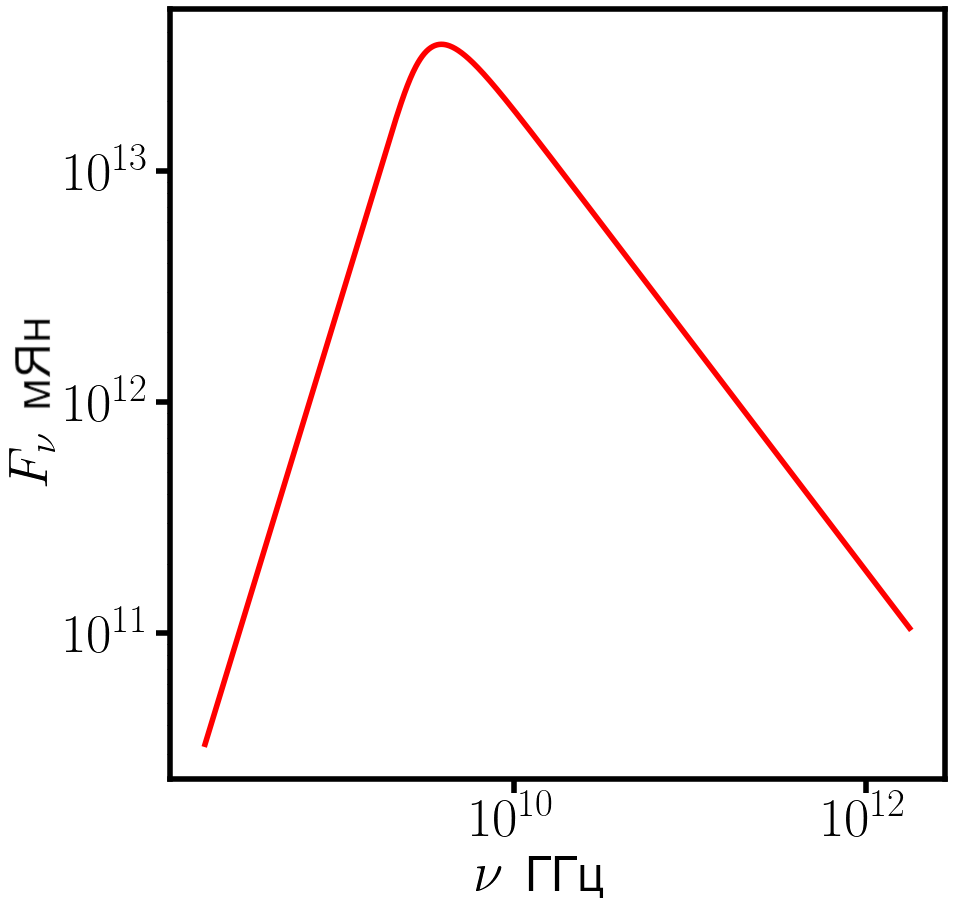
\includegraphics[width=12.5 cm]{./fig/example0.png} 
	\caption{Synchrotron radiation flux energy density from test source}
	\label{example0}
\end{figure}
	% Введение
	\chapter{Evaluation the radiation of the sources}\label{radiation}
FAINA allows to evaluate electromagnetic radiation from sources with various type of particle distributions and different parameters such ass magnetic fiels, number density and other. In current version of the code following types of radiation are implemented: synchrotron radiation, inverse Compton scattering, gamma-ray emission due to pion decay in free-free proton interaction and also bremsstrahlung.

\section{Particle distributions}

Crucial parameter for evaluation of any type of radiation is a distribution function of emitting particles. In the FAINA code abstract class ParticleDistribution and derived classes are used for representation of distributions. Public methods of class ParticleDistribution are listed in Table \ref{ParticleDistribution}:

\begin{small}
		\topcaption{Public methods of ParticleDistribution class}
		\label{ParticleDistribution}
		
		\begin{xtabular}{|p{0.45\textwidth}|p{0.55\textwidth}|}
			\hline
			\textbf{ParticleDistribution} & abstract class for particle distributions\\
			\hline
			double distribution(const double\& energy, const double\& mu, const double\& phi) & returns probability density function in polar coordinates with given energy, cosinus of polar angle and azimutal angle, normalized to the particles number density \\
			\hline
			virtual double distributionNormalized(const double\& energy, const double\& mu, const double\& phi) & virtual method, returns probability density function in polar coordinates with given energy, cosinus of polar angle and azimutal angle, normalized to unity\\
			\hline
			virtual double getMeanEnergy() & virtual method, returns mean energy of particles in distribution\\
			\hline
			double getConcentration() & returns particles number density\\
			\hline
			void resetConcentration(const double\& concentration) & changes number density to the given value\\
			\hline
		\end{xtabular}
\end{small}

For creating a distribution object you need some inherited class. Inheritance tree of ParticleDistribution splits into two big branches - PhotonDistribution for distribution of photons, and MassiveParticleDistribution - for massive particles. Scheme of class hierarchy is shown in Figure  \ref{particleDistribution0}. 

\begin{figure}
	\centering
	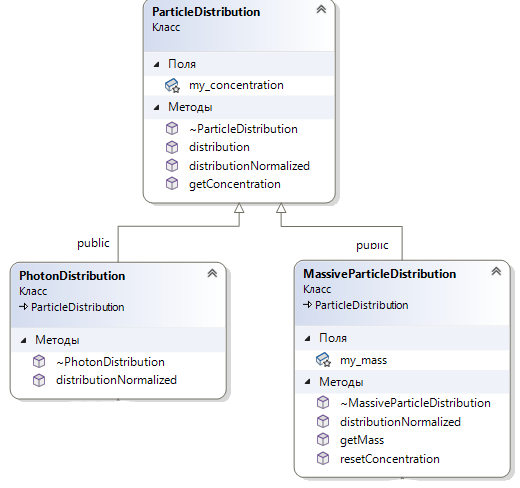
\includegraphics[width=8.5 cm]{./fig/particleDistribution0.png} 
	\caption{Two branches of inheritance tree of ParticleDIstribution}
	\label{particleDistribution0}
\end{figure}

It is important to note, that photons distributions are not used to represent results of evaluation of electromagnetic radiation. They are necessary only as input parameter for evaluation of inverse Compton scattering. Class PhotonDistribution is only an interface and has not its own specific methods. Class MassiveParticleDistribution is also abstract, but his methods are listed in Table \ref{MassiveParticleDistribution}	
\begin{small}
		\topcaption{Public methos of MassiveParticleDistribution class}
		\label{MassiveParticleDistribution}
		
			\begin{xtabular}{|p{0.45\textwidth}|p{0.55\textwidth}|}
				\hline
				\textbf{MassiveParticleDistribution} & abstract class for massive particles distribution\\
				\hline
				virtual double minEnergy() & virtual method, returns the lowest possible energy of particle in this distribution\\
				\hline
				virtual double maxEnergy() & 
				virtual method, returns the upper limit of energy of particle in this distribution. NOTE that if upper limit of energy is infinite, this method returns negative number\\
				\hline
				double getMass() & returns mass of single particle \\
				\hline
			\end{xtabular}
		\end{small}
\subsection{Photon distributions}

Abstract class PhotonDistribution has following derived class: abstract PhotonIsotropicDistribution, which represented isotopic distributions and some non-abstract classes: PhotonPlankDirectedDistribution, which represent photons with Plank distribution with respect to energy, but collimated in some solid angle, and CompoundPhotonDistribution, which is usefull for sum of several arbitrary photon distributions.

Class PhotonIsotropicDistribution again has its own inherited classes. It is a PhotonPowerLawDistribution for powerlaw distribution, PhotonPlankDistribution for Plank distributions, PhotonMultiPlankDistribution for sum of several Plank distributions and PhotonMonoenergeticDistribution for isotropic photons with same energy. Class hoerarchy of photon distributions is presented in Figure \ref{photonDistribution}.

\begin{figure}
	\centering
	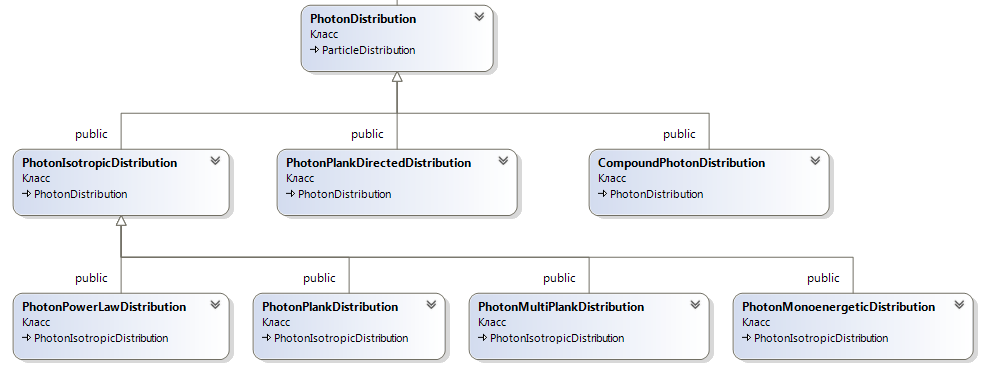
\includegraphics[width=10.5 cm]{./fig/photonDistribution2.png} 
	\caption{Class hierarchy of photon distributions}
	\label{photonDistribution}
\end{figure}

Methods of PhotonDistribution and it's inherited classes are listed in Table \ref{photonDistributionMethods}. NOTE, that metods distributionNormalized(const double\& energy) and distribution(const double\& energy) are not distribution with respect to energy, but just full distribution with dropped angular arguments. So to obtain distribution with respect to energy one should multiply result of this functions by $4\pi$.


\begin{small}
	\topcaption{Public methods of PhotonDistribution class and derived classes}
	\label{photonDistributionMethods}
	\begin{xtabular}{|p{0.45\textwidth}|p{0.55\textwidth}|}
				\hline
				\textbf{PhotonDistribution} & abstract interface for photon distributions\\
				\hline
				\textbf{PhotonIsotropicDistribution} & abstract class for isotropic distributions of photons\\
				\hline
				double distribution(const double\& energy) & returns probability density function in polar coordinates with dropped angular arguments (normalized to the number density divided by $4\pi$)\\
				\hline
				virtual double distributionNormalized(const double\& energy) & virtual method, returns probability density function in polar coordinates with dropped angular arguments (mormalized to the $1/4\pi$)\\
				\hline
				void writeDistribution(const char* fileName, int Ne, const double\& Emin, const double\& Emax) & записывает распределение в файл в виде двух столбцов с точками распределенными логарифмически\\
				\hline
				\textbf{PhotonPowerLawDistribution} & Класс для степенного распределения фотонов\\
				\hline
				PhotonPowerLawDistribution(const double\& index, const double\& E0, const double\& concentration) & конструктор, создающий экземпляр с заданными показателем наклона, начальной энергией и полной концентрацией \\
				\hline
				double getIndex() & возвращает показатель наклона спектра\\
				\hline
				double getE0() & возвращает минимальную энергию степенного распределения\\
				\hline
				\textbf{PhotonPlankDistribution} & Класс для планковского распределения фотонов\\
				\hline
				PhotonPlankDistribution(const double\& temperature, const double\& amplitude) & конструктор, создающий экземпляр с заданными температурой и апмплитудой - то есть отношением концентрации к равновесному планковскому распределению с данной температурой\\
				\hline
				static PhotonPlankDistribution* getCMBRadiation() & статический метод, возвращающий экземпляр, соответствующий реликтовому излучению (температура $2.725 K$, амплитуда $1$)\\
				\hline
				double getTemperature() & возвращает температуру распределения\\
				\hline
				\textbf{PhotonMultiPlankDistribution} & Класс для распределения фотонов, состоящего из суммы планковских распределений\\
				\hline
				PhotonMultiPlankDistribution(int Nplank, const double* const temperatures, const double* const amplitudes) & конструктор, принимающий количество планковских распределений, участвующих в смеси, массив их температур и массив амплитуд\\
				\hline
				static PhotonMultiPlankDistribution* getGalacticField() & статический метод, возвращающий экземпляр, соответствующий среднегалактическому фотонному распределению, по данным статьи \cite{Mathis1983}. Данное распределение состоит из пяти планковских компонент, с температурами $2.725K, 20K, 3000K, 4000K, 7000K$ и амплитудами $1.0, 4\cdot10^{4}, 4\cdot10^{-13}, 1.65\cdot10^{-13}, 1.0\cdot10^{-14}$ соответственно\\
				\hline
				\textbf{PhotonMonoenergeticDistribution} & Класс для моноэнергетического изотропного распределения фотонов\\
				\hline
				PhotonMonoenergeticDistribution(const double\& Energy, const double\& halfWidth, const double\& concentration) & конструктор, принимающий среднюю энергию распределения, полуширину разброса вокруг нее и концентрацию\\
				\hline
				\textbf{CompoundPhotonDistribution} & Класс для распределения фотонов, состоящего из суммы других распределений\\
				\hline
				CompoundPhotonDistribution(int N, PhotonDistribution** distributions) & конструктор, создающий экземпляр с заданным количеством распределений в смеси и массивом этих распределений \\
				\hline
				CompoundPhotonDistribution( PhotonDistribution* dist1, PhotonDistribution* dist2) & конструктор, создающий экземпляр содержащий смесь из двух распределений\\
				\hline
				CompoundPhotonDistribution( PhotonDistribution* dist1, PhotonDistribution* dist2, PhotonDistribution* dist3) & конструкторб создающий экземпляр содержащий смесь из трех распределений\\
				\hline
				\textbf{PhotonPlankDirectedDistribution} & Класс для направленного планковского распределения фотонов\\
				\hline
				PhotonPlankDirectedDistribution(const double\& temperature, const double\& amplitude, const double\& theta0, const double\& phi0, const double\& deltaTheta) & конструктор, принимающий температуру, амплитуду, углы задающие направление излучения и угол задающий полуширину раствора конуса излучения\\
				\hline
				double getTemperature() & возвращает температуру распределения\\
				\hline
	\end{xtabular}
\end{small}

Класс CompoundPhotonDistribution предназначен для представления смеси различных распределений фотонов, не обязательно планковских, как PhotonMultiPlankDistribution, и не обязательно изотропных. Его методы описаны в Таблице \ref{CompoundPhotonMethods}


Единственное реализованное в коде анизотропное распределение фотонов - это PhotonPlankDirectedDistribution, представляющий направленное планковское излучение. Пользователь может реализовать другие виды анизотропных излучений самостоятельно, создав класс, наследующий от PhotonDistribution и определив необходимый виртуальный метод distributionNormalized(const double\& energy, const double\& mu, const double\& phi). Методы класса PhotonPlankDirectedDistribution описаны в Таблице \ref{PhotonPlankDirectedDistributionMethods}


\subsection{Распределения массивных частиц}
Распределения массивных частиц представлены наследниками класса MassiveParticleDistribution. Так же как и в случае с фотонами важную роль играет абстрактный клас для представления изотропных распределений - MassiveParticleIsotropicDistribution. У этого класса есть методы возвращающие значение функции распределения в зависимости от энергии, и опять же, это не функция распределения, проинтегрированная по углам, а полная функция распределения с отброшенными угловыми аргументами. Для получения значения функции распределения по энергии нужно домножить значение, возвращенное данным методом на $4 \pi$. 

\begin{small}
		\topcaption{Публичные методы класса MassiveParticleIsotropicDistribution }
		\label{MassiveParticleMethods}
			\begin{xtabular}{|p{0.45\textwidth}|p{0.55\textwidth}|}
				\hline
				\textbf{MassiveParticleIsotropicDistribution} & Абстрактный класс для изотропных распределений\\
				\hline
				double distribution(const double\& energy) & возвращает функцию распределения с отброшенными угловыми аргументами, то есть нормированную на концентрацию, деленную на $4 \pi$ \\
				\hline
				virtual double distributionNormalized(const double\& energy) & чисто виртуальный метод, возвращает функцию распределения с отброшенными угловыми аргументами, нормированную на  $ 1 / 4 \pi$\\
				\hline
				void writeDistribution(const char* fileName, int Ne, const double\& Emin, const double\& Emax) & записывает распределение в файл с данным именем, в диапазоне межджу данными минимальной и максимальной енергиями с заданным количеством точек, которые распределяются логарифмически\\
				\hline
	\end{xtabular}
\end{small}

\begin{figure}[h]
	\centering
	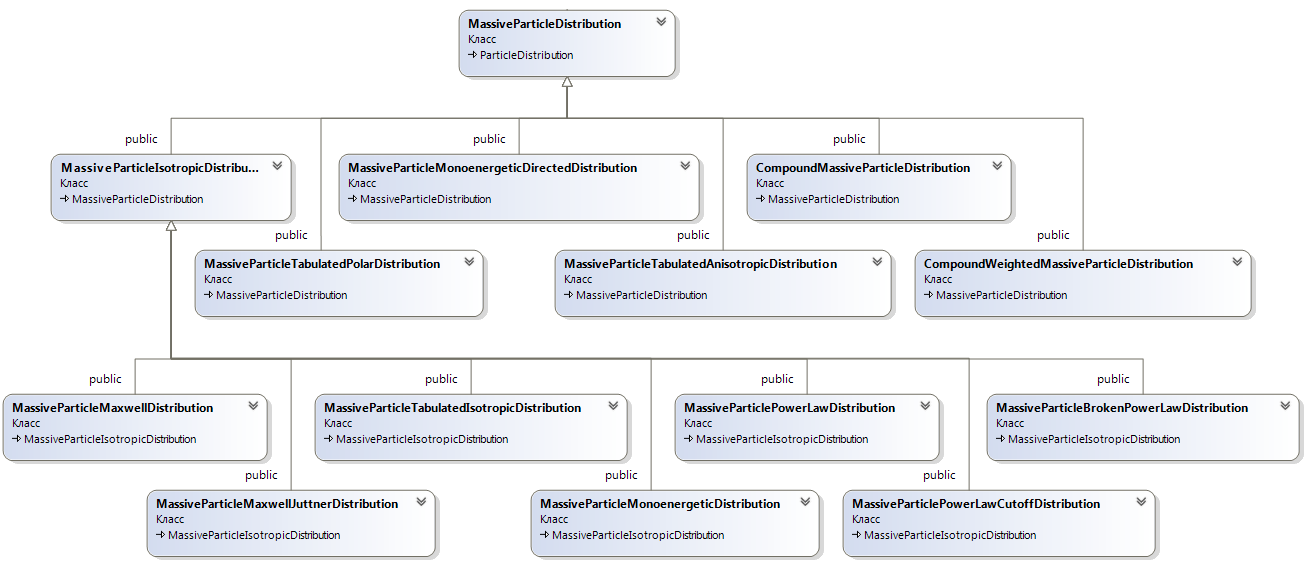
\includegraphics[width=14.5 cm]{./fig/massiveParticleDistribution2.png} 
	\caption{Схема наследования классов распределения массивных частиц}
	\label{massiveDistribution}
\end{figure}

Абстрактный класс изотропных распределений имеет семь наследников, предназначенных для создания конкретных распределений: MassiveParticlePowerLawDistribution - для степенных распределений, MassiveParticleBrokenPowerLawDistribution - для степенных распределений с изломом, MassiveParticlePowerLawCutoffDistribution - для степенных распределений с экспоненциальным завалом, MassiveParticleMaxwellDistribution - для максвелловского распределения (обратите внимание, что в отличие от остальных распределений, максвелловское подразумевает под энергией только кинетическую энергию), MassiveParticleMaxwellJuttnerDistribution - для релятивистского распределения Максвелла-Юттнера, MassiveParticleTabulatedIsotropicDistribution - для таблично заданных распределений и MassiveParticleMonoenergeticDistribution - для моноэнергичного изотропного распределения.

Так же имеется шесть реализаций анизотропных распределений: MassiveParticleTabulatedPolarDistribution - для таблично заданных распределений с зависимостью только от энергии и полярного угла, MassiveParticleAnisotropicDistribution - для таблично заданных распределений с зависимостью от всех переменных, MassiveParticleMonoenergeticDirectedDistribution - для моноэнергичного пучка частиц, с импульсами направленными в заданный телесный угол, MassiveParticleMovingDistribution - для перевода функций распределения в движущуюся систему отсчета, CompoundMassiveParticleDistribution - для суммы распредлений общего вида, CompoundWeightedMassiveParticleDistribution - для взвешенной суммы распределений общего вида. В некоторых случаях оперировать весами распределений удобнее, чем непосредственно концентрациями. Полная схема наследования классов распределений массивных частиц представлена на рисунке \ref{massiveDistribution}, список публичных методов классов распределений массивных частиц приведен в Таблице \ref{MassiveParticleMethods1}. Пользователь может сам реализовывать необходимые ему виды распределений излучающих частиц, создав наследника класса MassiveParticleDistribution или MassiveParticleIsotropicDistribution и определив необходимые виртуальные методы.

\subsection{Считывание распределений из файла}
Классы таблично-заданных распределений, такие как например MassiveParticleTabulatedIsotropicDistribution, имеют конструктор принимающие на вход имена файлов, из которых будет считана функция распределения. Это должны быть текстовые файлы, содержащие таблицы с данными, причем формат единиц, в которых измеряется функция распределения может быть разным. Для задания формата входных файлов используется перечислимы тип DistributionInputType, имеющий пять значений:

\begin{itemize}
	\item ENERGY\_FE - во входных файлах заданы энергия и функция распределения по энергии
	\item ENERGY\_KIN\_FE - заданы кинетическая энергия и функция распределения по энергии
	\item GAMMA\_FGAMMA - задан лоренц-фактор и функция распределения по нему
	\item GAMMA\_KIN\_FGAMMA - задан лоренц-фактор, уменьшенный на единицу, и функция распределения по нему
	\item MOMENTUM\_FP - задан импульс и функция распределения по импульсу
\end{itemize}

Вне зависимости от формата входного файла, функция распределения будет преобразована к единицам энергия - распределение по энергии. С помощью этих параметров можно считывать табличные распределения из файлов, например так:

\begin{lstlisting}[language=c++]
	double electronConcentration = 1.0;
	int N = 100;
	MassiveParticleIsotropicDistribution* distribution = new
	MassiveParticleTabulatedIsotropicDistribution(massElectron,
	"energy.dat", "distribution.dat", N, electronConcentration,
	DistributionInputType::ENERGY_FE);
\end{lstlisting}

Для облегчения создания распределений из файла в сложных случаях реализован класс MassiveParticleDistributionFactory. У него есть несколько методов, позволяющих считывать целые серии распределений из набора пронумерованных файлов. Что может быть полезно, если функция распределения зависит от некоторого параметра, как в примере вычисления синхротронного излучения описанном в следующей главе \ref{}. Считать серию из десяти распределений электронов, содержащихся в файлах с именами  "Fe0.dat"\ , "Fe1.dat"\  и так далее, состоящих из двух колонок - лоренц-фактор и функция распределения, и добавить к этим распределениям степенной хвост с показателем 3, начиная с энергий в 100 энергий покоя можно вызовом одной функции: 

\begin{lstlisting}[language=c++]
	double electronConcentration = 1.0;
	int Nenergy = 100;
	int Ndistribution = 100;
	double powerLawEnergy = 100*me_c2;
	double index = 3.0;
	MassiveParticleIsotropicDistribution** distributions = 
	MassiveParticleDistributionFactory::
	readTabulatedIsotropicDistributionsAddPowerLawTail(
	massElectron, "./input/Fe", ".dat", Ndistribution, 
	DistributionInputType::GAMMA_FGAMMA, electronConcentration, Nenergy,
	powerLawEnergy, index);
\end{lstlisting}

Так же у пользователя есть возможность использовать конструкторы табличных распределений, принимающие не имена файлов, а непосредственно массивы со значениями функции распределения, которые пользователь может создать любым удобным ему способом.

\begin{small}
	\topcaption{Публичные методы классов распределений массивных частиц }
	\label{MassiveParticleMethods1}
	\begin{xtabular}{|p{0.52\textwidth}|p{0.48\textwidth}|}
		\hline
		\textbf{MassiveParticlePowerLawDistribution} & Класс для степенного распределения\\
		\hline
		MassiveParticlePowerLawDistribution( const double\& mass, const double\& index, const double\& E0, const double\& concentration) & конструктор, создает экземпляр степенного распределния частиц с заданными массой, степенным индексом, начальной энергией распределения и полной концентрацией\\
		\hline
		double getIndex() & возвращает степенной индекс распределения\\
		\hline
		double getE0() & возвращает начальную энергию распределения\\
		\hline
		\textbf{MassiveParticleBrokenPowerLawDistribution} & Класс для степенного распределения с изломом\\
		\hline
		MassiveParticleBrokenPowerLawDistribution( const double\& mass, const double\& index1, const double\& index2, const double\& E0, const double\& Etran, const double\& concentration) & конструктор, создает экземпляр степенного распределния с изломом частиц с заданными массой, степенными индексоми на низких и высоких энергиях, начальной энергией распределения, энергией соответствующей излому и полной концентрацией\\
		\hline
		double getIndex1() & возвращает степенной индекс распределения на низких энергиях\\
		\hline
		double getIndex2() & возвращает степенной индекс распределения на высоких энергиях\\
		\hline
		double getE0() & возвращает начальную энергию распределения\\
		\hline
		double getEtran() & возвращает энергию излома\\
		\hline
		\textbf{MassiveParticlePowerLawCutoffDistribution} & Класс для степенного распределения с экспоненциальным завалом\\
		\hline
		MassiveParticlePowerLawCutoffDistribution(const double\& mass, const double\& index, const double\& E0, const double\& beta, const double\& Ecut, const double\& concentration) & конструктор, создает экземпляр степенного распределния с экспоненциальным завалом частиц с заданными массой, степенным индексом, начальной энергией распределения, параметром завала, энергией завала и полной концентрацией. $F(E)\propto (E/E_0)^{-index}\cdot\exp(-(E/E_{cut})^\beta)$\\
		\hline
		double getIndex() & возвращает степенной индекс распределения \\
		\hline
		double getBeta() & возвращает параметр завала распределения \\
		\hline
		double getE0() & возвращает начальную энергию распределения\\
		\hline
		double getEcutoff() & возвращает энергию экспоненциального завала\\
		\hline
		\textbf{MassiveParticleMaxwellDistribution} & Класс для распределения Максвелла\\
		\hline
		MassiveParticleMaxwellDistribution( const double\& mass, const double\& temperature, const double\& concentration) & конструктор, создает экземпляр распределния Максвелла частиц с заданными массой, температурой и полной концентрацией\\
		\hline
		double getTemperature() & возвращает температуру распределения\\
		\hline
		\textbf{MassiveParticleMaxwellJuttnerDistribution} & Класс для распределения Максвелла-Юттнера\\
		\hline
		MassiveParticleMaxwellJuttnerDistribution( const double\& mass, const double\& temperature, const double\& concentration) & конструктор, создает экземпляр распределния Максвелла-Юттнера частиц с заданными массой, температурой и полной концентрацией\\
		\hline
		double getTemperature() & возвращает температуру распределения\\
		\hline
		\textbf{MassiveParticleTabulatedIsotropicDistribution} & Класс для таблично заданного изотропного распределения\\
		\hline
		MassiveParticleTabulatedIsotropicDistribution( const double\& mass, const char* fileName, const int N, const double\& concentration, DistributionInputType inputType) & конструктор, создает экземпляр табличного распределния частиц с заданными массой и полной концентрацией с помощью указанного файла, состоящего из двух колнок с данными указанной длины. Так же указывается формат входных данных.\\
		\hline
		MassiveParticleTabulatedIsotropicDistribution( const double\& mass, const char* energyFileName, const char* distributionFileName, const int N, const double\& concentration, DistributionInputType inputType) & конструктор, создает экземпляр табличного распределния частиц с заданными массой и полной концентрацией с помощью указанных двух файлов, состоящих из колнок с данными указанной длины. Так же указывается формат входных данных. \\
		\hline
		MassiveParticleTabulatedIsotropicDistribution( const double\& mass, const double* energy, const double* distribution, const int N, const double\& concentration, DistributionInputType inputType) & конструктор, создает экземпляр табличного распределния частиц с заданными массой и полной концентрацией с помощью двух переданных массивов данных указанной длины. Так же указывается формат входных данных.\\
		\hline
		int getN() & возвращает количество ячеек в таблице задающей функцию\\
		\hline
		double getEmin() & возвращает минимальную энергию распределения\\
		\hline
		double getEmax() & возвращает максимальную энергию распределения\\
		\hline
		double rescaleDistribution(const double\& k) & масштабирует распределение, вытягивая его по оси энергии по формуле $E' = mc^2 + k\cdot(E-mc^2)$, $F(E')=F(E)/k$. Данная функция может быть полезна, например, в случае когда исходная функция распределения получена в результате работы численного кода с измененной массой электронов\\
		\hline
		void addPowerLaw( const double\& Epower, const double\& index) & добавляет к функции распределения степенной с указанным индексом, начиная с указанной энергии. Функция распределения при этом остается нормированной на указанную ранее концентрацию\\
		\hline
		\textbf{MassiveParticleMonoenergeticDistribution} & Класс для моноэнергичного изотропного распределения\\
		\hline
		MassiveParticleMonoenergeticDistribution(const double\& mass, const double\& Energy, const double\& halfWidth, const double\& concentration) & конструктор, принимающий массу, среднюю энергию, полуширину разброса по энергии и концентрацию\\
		\hline 
		\textbf{MassiveParticleTabulatedPolarDistribution} & Класс для таблично заданного распределения с зависимостью от полярного угла\\
		\hline
		MassiveParticleTabulatedPolarDistribution( const double\& mass, const char* energyFileName, const char* muFileName, const char* distributionFileName, const int Ne, const int Nmu, const double\& concentration, DistributionInputType inputType) & конструктор, создает экземпляр табличного распределния частиц с заданными массой и полной концентрацией с помощью  трех указанных файлов, в двух из которых содержатся сетки по энергии и косинусу полярного угла с указанными размерами, а в третьем двумерный массив функции распределения. Так же указывается формат входных данных.\\
		\hline
		MassiveParticleTabulatedPolarDistribution( const double\& mass, const double* energy, const double* mu, const double** distribution, const int Ne, const int Nmu, const double\& concentration, DistributionInputType inputType) & конструктор, создает экземпляр табличного распределния частиц с заданными массой и полной концентрацией с помощью трех переданных массивов данных, в двух из которых содержатся сетки по энергии и косинусу полярного угла с указанными размерами, а в третьем двумерный массив функции распределения. Так же указывается формат входных данных.\\
		\hline
		int getNe() & возвращает количество ячеек по энергии в таблице задающей функцию распределения\\
		\hline
		double getEmin() & возвращает минимальную энергию распределения\\
		\hline
		double getEmax() & возвращает максимальную энергию распределения\\
		\hline
		int getNmu() & возвращает количество ячеек по полярному углу в таблице задающей функцию распределения\\
		\hline
		void double rescaleDistribution(const double\& k) & масштабирует распределение, вытягивая его по оси энергии по формуле $E' = mc^2 + k\cdot(E-mc^2)$, $F(E',\mu)=F(E,\mu)/k$. Данная функция может быть полезна, например, в случае когда исходная функция распределения получена в результате работы численного кода с измененной массой электронов\\
		\hline
		\textbf{MassiveParticleTabulatedAnisotropicDistribution} & Класс для таблично заданного анизотропного распределения общего вида\\
		\hline
		MassiveParticleTabulatedAnisotropicDistribution( const double\& mass, const char* energyFileName, const char* muFileName, const char* distributionFileName, const int Ne, const int Nmu, const int Nphi, const double\& concentration, DistributionInputType inputType) & конструктор, создает экземпляр табличного распределния частиц с заданными массой и полной концентрацией с помощью  трех указанных файлов, в двух из которых содержатся сетки по энергии и косинусу полярного угла с указанными размерами, а в третьем двумерный массив функции распределения. Сетка по азимутальному углу считается расномерной и определяется только размером. Так же указывается формат входных данных.\\
		\hline
		MassiveParticleTabulatedAnisotropicDistribution( const double\& mass, const double* energy, const double* mu, const double*** distribution, const int Ne, const int Nmu, const int Nphi, const double\& concentration, DistributionInputType inputType) & конструктор, создает экземпляр табличного распределния частиц с заданными массой и полной концентрацией с помощью трех переданных массивов данных, в двух из которых содержатся сетки по энергии и косинусу полярного угла с указанными размерами, а в третьем двумерный массив функции распределения. Сетка по азимутальному углу считается расномерной и определяется только размером. Так же указывается формат входных данных.\\
		\hline
		int getNe() & возвращает количество ячеек по энергии в таблице задающей функцию распределения\\
		\hline
		double getEmin() & возвращает минимальную энергию распределения\\
		\hline
		double getEmax() & возвращает максимальную энергию распределения\\
		\hline
		int getNmu() & возвращает количество ячеек по полярному углу в таблице задающей функцию распределения\\
		\hline
		int getNphi() & возвращает количество ячеек по азимутальному углу в таблице задающей функцию распределения\\
		\hline
		void rescaleDistribution(const double\& k) & масштабирует распределение, вытягивая его по оси энергии по формуле $E' = mc^2 + k\cdot(E-mc^2)$, $F(E',\mu, \phi)=F(E,\mu, \phi)/k$. Данная функция может быть полезна, например, в случае когда исходная функция распределения получена в результате работы численного кода с измененной массой электронов\\
		\hline
		\textbf{MassiveParticleMonoenergeticDirectedDistribution} & Класс для моноэнергичного направленного пучка частиц\\
		\hline
		MassiveParticleMonoenergeticDirectedDistribution(const double\& mass, const double\& Energy, const double\& halfWidth, const double\& concentration, const double\& theta0, const double\& phi0, const double\& deltaTheta) & конструктор, принимающий массу частиц, среднюю энергию, полуширину разброса, концентрацию, углы задающие направление пучка и угол полуширины раствора конуса\\
		\hline
		\textbf{MassiveParticleMovingDistribution} & Класс осуществляющий перевод функций распределения в движущуюся систему отсчета\\
		\hline
		MassiveParticleMovingDistribution( MassiveParticleDistribution* distribution, const double\& velocity) & конструктор, принимающий функцию распределения в собственной системе отсчета и скорость движения этой системы вдоль оси z относительно лабораторной системы\\
		\hline
		\textbf{CompoundMassiveParticleDistribution} & Класс для распределения, состоящего из суммы других распределений\\
		\hline
		CompoundMassiveParticleDistribution( int N, MassiveParticleDistribution** distributions) & конструктор, создает экземпляр класса содержащий смесь заданного количества указанных распределений\\
		\hline
		CompoundMassiveParticleDistribution( MassiveParticleDistribution* dist1, MassiveParticleDistribution* dist2) & конструктор, создает экземпляр класса, содержащий смесь двух распределений \\
		\hline
		CompoundMassiveParticleDistribution( MassiveParticleDistribution* dist1, MassiveParticleDistribution* dist2, MassiveParticleDistribution* dist3) & конструктор, создает экземпляр класса, содержащий смесь трех распределений\\
		\hline
		\textbf{CompoundWeightedMassiveParticleDistribution} & Класс для распределения, состоящего из взвешенной суммы других распределений \\
		\hline
		CompoundWeightedMassiveParticleDistribution( int N, const double* weights, MassiveParticleDistribution** distributions) & конструктор, создает экземпляр класса содержащий смесь заданного количества указанных распределений с заданными весами \\
		\hline
		CompoundWeightedMassiveParticleDistribution( MassiveParticleDistribution* dist1, const double\& w1, MassiveParticleDistribution* dist2, const double\& w2) & конструктор, создает экземпляр класса, содержащий смесь двух распределений с указанными весами \\
		\hline
		CompoundWeightedMassiveParticleDistribution( MassiveParticleDistribution* dist1, const double\& w1, MassiveParticleDistribution* dist2, const double\& w2, MassiveParticleDistribution* dist3, const double\& w3) & конструктор, создает экземпляр класса, содержащий смесь трех распределений с указанными весами \\
		\hline
				
	\end{xtabular}
\end{small}

\section{Источники излучения}

В коде FAINA есть возможность расчета излучения, используя на прямую функции распределения излучающих частиц, с указанием необходимых дополнительных параметров, таких как объем источника, расстояние до него, магнитное поле и других. Но более универсальным и рекомендованным способ является расчет с помощью создания модели источника излучения. При таком подходе возможно учесть геометрическое строение источника, его неоднородности и другие особенности.

Реализованы два базовых класса источников - независящие от времени, представленные абстрактным классом RadiationSource, и изменяющиеся со временем, представленные абстрактным классом RadiationTimeDependentSource. Эти два класса не связаны между собой через наследование, но объект первого класса содержится внутри объектов второго как приватное поле класса. Схема классов источников излучения представлена на рисунке \ref{radiationSource}.

\begin{figure}[h]
	\centering
	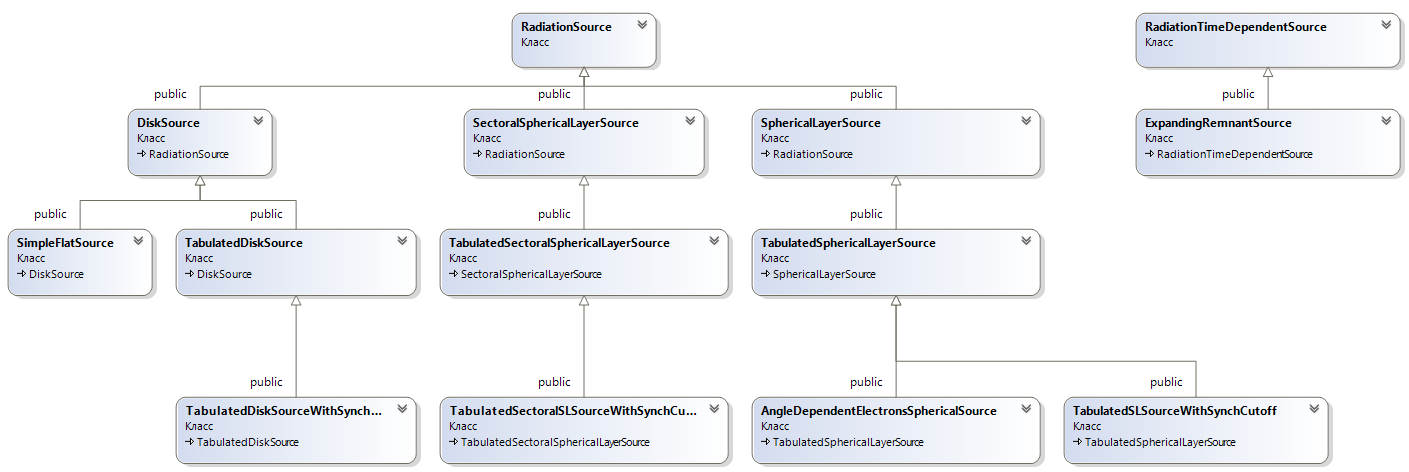
\includegraphics[width=14.5 cm]{./fig/radiationSource2.png} 
	\caption{Схема наследования классов источников излучения}
	\label{radiationSource}
\end{figure}

\subsection{Источники излучения, не зависящие от времени}\label{sourcesSection}
Источники излучения без временной зависимости реализованы с помощью абстрактного класса RadiationSource. Геометрически каждый источник задан в виде пространственной области в цилиндрических координатах, с осью z направленной вдоль луча зрения к наблюдателю, и характеризуется максимальным радиусом и минимальным и максимальным значением координаты z. Такая система координат выбрана для удобства учета процессов поглощения при прохождении излучения внутри самого источника вдоль луча зрения. Отличие реальной формы источника от цилиндрической реализовано с помощью долей заполнения веществом источника ячеек пространственной сетки. Модель источника, имеющего форму шарового слоя, в цилиндрическо пространственной сетке изображена на рисунке \ref{sphericalLayer}. Цветом обозначена доля объема ячейки, заполненная веществом источника.

\begin{figure}
	\centering
	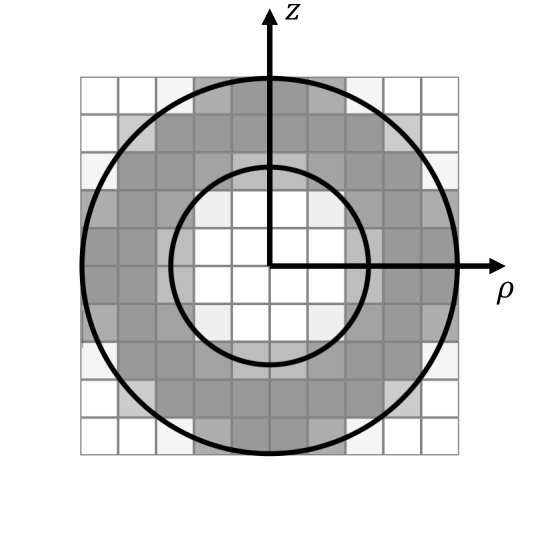
\includegraphics[width=10.5 cm]{./fig/sphericalSource.png} 
	\caption{Модель источника в форме шарового слоя, помещенного в цилиндрическую пространственную координатную сетку. Цвет характеризует долю объема ячейки, заполненную веществом источника.}
	\label{sphericalLayer}
\end{figure}

Так же источники излучения имеют следующие важные характеристки, которые могут меняться в различных пространственных ячейках источника: концентрация излучающих частиц, их функция распределения, магнитное поле и угол его наклона к лучу зрения. Большинство методов расчета излучения (все кроме обратного комптоновского рассеяния) реализованы только для изотропных распределений излучающих частиц, поэтому источники содержат только изотропные распределения. Так же у источника должно быть задано расстояние до наблюдателя.

Класс RadiationSource имеет три абстрактных класса-наследника: DiskSource - для источников в форме диска, перпендикулярного лучу зрения, и SphericalLayerSource - для источников в форме шарового слоя и SectoralSphericalLayerSource - источник, который нужен тогда, когда рассматривается только сектор шарового слоя, "долька апельсина". 

Источники в форме диска имеют три реализации: SimpleFlatSource - однородный диск, состоящий из одной пространственной ячейки с заданными параметрами, и TabulatedDiskSource - источник, в котором все характеристики таблично заданы на пространственной сетке и отнаследованный от него TabulatedDiskSourceWithSynchCutoff, который нужен для учета синхротронных потерь функции распределения. В можели данного источника считается, что распределение частиц генерирутся на границе источника (верхней грани, соответствующей ударной волне), а в дальнейшем конвекционно переносятся вглубь него, испытывая при этом синхротронные потери. Изменение функции распределения в зависимости от расстояния до границы в случае однородного поля определеяется формулой:

\begin{equation}
	f_l(E)=f\left(\frac{E}{1-4e^4 B^2 E~l/9m^4 c^7 v}\right)\cdot\frac{1}{\left(1-4e^4 B^2 E~l/9m^4 c^7 v\right)^2}
\end{equation}
где $f(E)$ исходная функция распределения, $E$ - энергия частицы, $B$ - магнитное поле, $l$ - расстояние до границы, $v$ - скорость конвекционного движения, $e$ - заряд частицы, $m$ - масса частицц, $c$ - скорость света.

Источники в форме шарового слоя имеют следующие реализации: TabulatedSphericalSource - источник, в котором все характеристики таблично заданы на пространственной сетке, и отнаследованные от него  TabulatedSLSourceWithSynchCutoff и AngleDependentElectronsSphericalSource. Первый из них нужен для учета синхротронных потерь, аналогично тому как это сделано в TabulatedDiskSourceWithSynchCutoff, а второй - для реализации важного случая, когда функция распределения излучающих частиц зависит от угла наклона магнитного поля по отношению к направлению распространения ударной волны \cite{SironiSpitkovsky2009pair, GuoSironi2014_1,Crumley2019, Romansky2018, еще}. В AngleDependentElectronsSphericalSource такие параметры, как концентрация, магнитное поле и его угол наклона к лучу зрения заданы таблично на пространственной сетке, а функция распределения излучающих частиц - в виде таблицы по углам наклона магнитного поля к направлению распространения ударной волны, которая в данном случае считается сферически симметричной. Функция распределения в каждой ячейке выбирается в зависимости от вычисленного угла наклона магнитного поля к ударной волне.

Источники в форме шарового слоя имеют следующие реализации: TabulatedSectoralSphericalLayerSource - источник, в котором все характеристики таблично заданы на пространственной сетке, и отнаследованный от него TabulatedSectoralSLSourceWithSynchCutoff, учитывающий потери энергии частиц аналогично тому, как это реализовано в классе TabulatedDiskSourceWithSynchCutoff.

Публичные методы классов источников излучения без зависимости от времени перечислены в Таблице \ref{sourceMethods1}.

\begin{small}
	\topcaption{Публичные методы классов источников излучения без зависимости от времени }
	\label{sourceMethods1}
	\begin{xtabular}{|p{0.5\textwidth}|p{0.5\textwidth}|}
		\hline
		\textbf{RadiationSource} & абстрактный класс для источников излучения общего вида\\
		\hline
		virtual double getMaxRho() & чисто виртуальный метод, возвращает границу источника по радиальной оси в цилиндрических координатах\\
		\hline
		virtual double getMinZ() & чисто виртуальный метод, возвращает минимальную границу источника по оси z\\
		\hline
		virtual double getMaxZ() & чисто виртуальный метод, возвращает максимальную границу источника по оси z\\
		\hline
		virtual double getMaxB() & чисто виртуальный метод, возвращает максимальное магнитное поле\\
		\hline
		virtual double getAverageSigma() & чисто виртуальный метод, возвращает среднюю магнетизацию $\sigma=\frac{B^2}{4\pi n m_p c^2}$\\
		\hline
		virtual double getAverageConcentration() &чисто виртуальный метод, возвращает среднюю конценрацию\\
		\hline
		virtual double getRho(int irho) & чисто виртуальный метод, возвращает радиальную координату данной ячейки\\
		\hline
		virtual double getZ(int iz)& чисто виртуальный метод, возвращает z координату данной ячейки\\
		\hline
		virtual double getPhi(int iphi)& чисто виртуальный метод, возвращает азимутальную координату данной ячейки\\
		\hline
		virtual int getRhoIndex(const double\& rho)& чисто виртуальный метод, возвращает радиальный индекс ячейки по координате\\
		\hline
		virtual bool isSource(int irho, int iphi)& чисто виртуальный метод, возвращает логическое значение - учитывать ли ячейки с данными радиальными и азимутальными координатами при расчете излучения всего источника\\
		\hline
		int getNrho() & возвращает количество пространственных ячеек по радиальной оси цилиндрических координат\\
		\hline
		int getNz() & возвращает количество пространственных ячеек по оси z цилиндрических координат\\
		\hline
		int getNphi() & возвращает количество пространственных ячеек по по азимутальному углу цилиндрических координат\\
		\hline
		double getDistance() & возвращает расстояние до источника\\
		\hline
		getArea(int irho) & возвращает поперечное сечение данной пространственной ячейки\\
		\hline
		getVolume(int irho, int iz, int iphi) & возвращает объем ячейки, занятый веществом источника. Этот метод согласован с методами getArea и getLength и возвращает их произведение\\
		\hline
		virtual getB(int irho, int iz, int iphi) & чисто виртуальный метод, возвращает значение магнитного поля в ячейке\\
		\hline
		virtual getConcentration(int irho, int iz, int iphi) & чисто виртуальный метод, возвращает значение концентрации в ячейке \\
		\hline
		virtual getSinTheta(int irho, int iz, int iphi) & чисто виртуальный метод, возвращает синус угла наклона магнитного поля к лучу зрения\\
		\hline
		virtual void getVelocity(int irho, int iz, int iphi, double\& velocity, double\& theta, double\& phi) &\\
		чисто виртуальный метод, возвращает скорость данной ячейки источника\\
		\hline
		virtual getTotalVolume() & чисто виртуальный метод, возвращает полный объем источника\\
		\hline
		virtual getLength(int irho, int iz, int iphi) & чисто виртуальный метод, возвращает среднюю толщину ячейки, заполненную веществом источника\\
		\hline
		virtual resetParameters(const double* parameters, const double* normalizationUnits) & чисто виртуальный метод, меняющий параметры источника. Список параметров, их количество, их влияние на источник определяются пользователем в конкретных реализациях класса. Принимет массив параметров и массив единиц в которых они измерены. Данный метод используется в процедурах оптимизации, либо при учете изменения источника со временем\\
		\hline
		virtual getParticleDistribution(int irho, int iz, int iphi) & чисто виртуальный метод, возвращает распределение излучающих частиц в ячейке\\
		\hline
		\textbf{DiskSource} & Абстрактный класс для источников в форме диска\\
		\hline
		\textbf{SimpleFlatSource} & Класс для источников в форме однородного диска\\
		\hline
		SimpleFlatSource( MassiveParticleDistribution* electronDistribution, const double\& B, const double\& sinTheta, const double\& rho, const double\& z, const double\& distance, const double\& velocity = 0) & конструктор, возвращает экземпляр с заданными распределением частиц, магнитным полем, синусом угла его наклона, радиусом диска, толщиной диска, расстоянием до источника и скоростью движения вещества\\
		\hline
		\textbf{TabulatedDiskSource} & Класс для источников в форме диска с таблично заданными значениями параметров\\
		\hline
		TabulatedDiskSource( int Nrho, int Nz, int Nphi, MassiveParticleDistribution* electronDistribution, double*** B, double*** sinTheta, double*** concentration, const double\& rho, const double\& z, const double\& distance, const double\& velocity = 0) & конструктор, возвращает экземпляр с заданными с помощью массивов распределением частиц, магнитным полем, синусом угла его наклона, а так же заданными радиусом диска, толщиной диска, расстоянием до источника и скоростью движения вещества\\
		\hline
		TabulatedDiskSource( int Nrho, int Nz, int Nphi, MassiveParticleDistribution* electronDistribution, const double\& B, const double\& sinTheta, const double\& concentration , const double\& rho, const double\& z, const double\& distance, const double\& velocity = 0) & конструктор, возвращает экземпляр с заданными однородными распределением частиц, магнитным полем, синусом угла его наклона, а так же заданными радиусом диска, толщиной диска, расстоянием до источника и скоростью движения вещества\\
		\hline
		\textbf{TabulatedDiskSourceWithSynchCutoff} & Класс для источников в форме диска с таблично заданными значениями параметров и учетом синхротронных потерь энергии частиц\\
		\hline
		TabulatedDiskSourceWithSynchCutoff(int Nrho, int Nz, int Nphi, MassiveParticleDistribution* electronDistribution, double*** B, double*** theta, double*** concentration, const double\& rho, const double\& z, const double\& distance, const double\& downstreamVelocity, const double\& velocity = 0) &
		конструктор, возвращает экземпляр с заданными с помощью массивов распределением частиц, магнитным полем, синусом угла его наклона, а так же заданными радиусом диска, толщиной диска, расстоянием до источника, скоростью конвекции частиц и скоростью движения вещества\\
		\hline
		TabulatedDiskSourceWithSynchCutoff(int Nrho, int Nz, int Nphi, MassiveParticleDistribution* electronDistribution, const double\& B, const double\& concentration, const double\& theta, const double\& rho, const double\& z, const double\& distance, const double\& downstreamVelocity, const double\& velocity = 0) & конструктор, возвращает экземпляр с заданными однородными распределением частиц, магнитным полем, синусом угла его наклона, а так же заданными радиусом диска, толщиной диска, расстоянием до источника, скоростью конвекции частиц и скоростью движения вещества\\
		\hline
		\textbf{SphericalLayerSource} & Абстрактный класс для источников в форме шарового слоя\\
		\hline
		double getInnerRho() & возвращает внутренний радиус шарового слоя\\
		\hline
		\textbf{TabulatedSphericalLayerSource} & Класс для источников в форме шарового слоя с таблично заданными значениями параметров\\
		\hline
		TabulatedSphericalLayerSource(int Nrho, int Nz, int Nphi, MassiveParticleDistribution* electronDistribution, double*** B, double*** sinTheta, double*** concentration, const double\& rho, const double\& rhoin, const double\& distance, const double\& velocity = 0) & конструктор, возвращает экземпляр с заданными с помощью массивов распределением частиц, магнитным полем, синусом угла его наклона к лучу зрения, а так же заданными внешним и внутренним радиусом шарового слоя, расстоянием до источника и скоростью движения вещества\\
		\hline
		TabulatedSphericalLayerSource(int Nrho, int Nz, int Nphi, MassiveParticleDistribution* electronDistribution, const double\& B, const double\& concentration, const double\& sinTheta, const double\& rho, const double\& rhoin, const double\& distance, const double\& velocity = 0) &  конструктор, возвращает экземпляр с заданными однородными распределением частиц, магнитным полем, синусом угла его наклона, а так же заданными внутренним и внешним радиусом шарового слоя, расстоянием до источника и скоростью движения вещества\\
		\hline
		\textbf{AngleDependentElectronsSphericalSource} & Класс для источников в форме шарового слоя с таблично заданными значениями концентрации и магнитного поля и функцией распределения излучающих частиц, зависящей от угла наклона магнитного поля к направлению распространения ударной волны\\
		\hline
		AngleDependentElectronsSphericalSource( int Nrho, int Nz, int Nphi, int Ntheta, MassiveParticleDistribution** electronDistributions, double*** B, double*** sinTheta, double*** phi, double*** concentration, const double\& rho, const double\& rhoin, const double\& distance, const double\& velocity = 0) & конструктор, возвращает экземпляр с заданными с помощью массивов магнитным полем, синусом угла его наклона к лучу зрения, а так же заданными внешним и внутренним радиусом шарового слоя, расстоянием до источника и скоростью движения вещества. Распределение частиц задается в виде массива табличных значений в зависимости от угла наклона магнитного поля к направлению распространения ударной волны\\
		\hline
		AngleDependentElectronsSphericalSource(int Nrho, int Nz, int Nphi, int Ntheta, MassiveParticleDistribution** electronDistributions, const double\& B, const double\& sinTheta, const double\& phi, const double\& concentration, const double\& rho, const double\& rhoin, const double\& distance, const double\& velocity = 0) & конструктор, возвращает экземпляр с заданными однородными  магнитным полем, синусом угла его наклона, а так же заданными внутренним и внешним радиусом шарового слоя, расстоянием до источника и скоростью движения вещества. Распределение частиц задается в виде массива табличных значений в зависимости от угла наклона магнитного поля к направлению распространения ударной волны\\
		\hline
		\textbf{TabulatedSLSourceWithSynchCutoff} & Класс для источников в форме шарового слоя с таблично заданными значениями параметров и учетом синхротронных потерь энергии частиц\\
		\hline
		TabulatedSLSourceWithSynchCutoff(int Nrho, int Nz, int Nphi, MassiveParticleDistribution* electronDistribution, double*** B, double*** theta, double*** concentration, const double\& rho, const double\& rhoin, const double\& distance, const double\& downstreamVelocity, const double\& velocity = 0) & конструктор, возвращает экземпляр с заданными с помощью массивов распределением частиц, магнитным полем, синусом угла его наклона к лучу зрения, а так же заданными внешним и внутренним радиусом шарового слоя, расстоянием до источника, скоростью конвекции частиц и скоростью движения вещества\\
		\hline
		TabulatedSLSourceWithSynchCutoff(int Nrho, int Nz, int Nphi, MassiveParticleDistribution* electronDistribution, const double\& B, const double\& concentration, const double\& theta, const double\& rho, const double\& rhoin, const double\& distance, const double\& downstreamVelocity, const double\& velocity = 0) & конструктор, возвращает экземпляр с заданными однородными распределением частиц, магнитным полем, синусом угла его наклона, а так же заданными внутренним и внешним радиусом шарового слоя, расстоянием до источника, скоростью конвекции частиц и скоростью движения вещества\\
		\hline
		\textbf{SectoralSphericalLayerSource} & абстрактный класс для источников в форме сектора шарового слоя (дольки апельсина)\\
		\hline
		double getRhoin() & возвращает внутренний радиус шарового слоя\\
		\hline
		\textbf{TabulatedSectoralSphericalLayerSource} & Класс для источников в форме сектора шарового слоя с таблично заданными значениями параметров\\
		\hline
		TabulatedSectoralSphericalLayerSource(int Nrho, int Nz, int Nphi, MassiveParticleDistribution* electronDistribution, double*** B, double*** theta, double*** concentration, const double\& rho, const double\& rhoin, const double\& minrho, const double\& phi, const double\& distance, const double\& velocity = 0) & конструктор, возвращает экземпляр с заданными с помощью массивов распределением частиц, магнитным полем, синусом угла его наклона к лучу зрения, а так же заданными внешним и внутренним радиусом шарового слоя, углом раствора сектора, расстоянием до источника и скоростью движения вещества\\
		TabulatedSectoralSphericalLayerSource(int Nrho, int Nz, int Nphi, MassiveParticleDistribution* electronDistribution, const double\& B, const double\& concentration, const double\& theta, const double\& rho, const double\& rhoin, const double\& minrho, const double\& phi, const double\& distance, const double\& velocity = 0) & конструктор, возвращает экземпляр с заданными однородными распределением частиц, магнитным полем, синусом угла его наклона, а так же заданными внутренним и внешним радиусом шарового слоя, углом раствора сектора, расстоянием до источника и скоростью движения вещества\\
		\hline
		\textbf{TabulatedSectoralSLSourceWithSynchCutoff} & Класс для источников в форме сектора шарового слоя с таблично заданными значениями параметров и учетом синхротронных потерь энергии частиц\\
		\hline
		TabulatedSectoralSLSourceWithSynchCutoff(int Nrho, int Nz, int Nphi, MassiveParticleDistribution* electronDistribution, double*** B, double*** theta, double*** concentration, const double\& rho, const double\& rhoin, const double\& minrho, const double\& phi, const double\& distance, const double\& downstreamVelocity, const double\& velocity = 0) & конструктор, возвращает экземпляр с заданными с помощью массивов распределением частиц, магнитным полем, синусом угла его наклона к лучу зрения, а так же заданными внешним и внутренним радиусом шарового слоя, углом раствора сектора, расстоянием до источника, скоростью конвекции частиц и скоростью движения вещества\\
		\hline
		TabulatedSectoralSLSourceWithSynchCutoff(int Nrho, int Nz, int Nphi, MassiveParticleDistribution* electronDistribution, const double\& B, const double\& concentration, const double\& theta, const double\& rho, const double\& rhoin, const double\& minrho, const double\& phi, const double\& distance, const double\& downstreamVelocity, const double\& velocity = 0) & конструктор, возвращает экземпляр с заданными однородными распределением частиц, магнитным полем, синусом угла его наклона, а так же заданными внутренним и внешним радиусом шарового слоя, углом раствора сектора, расстоянием до источника, скоростью конвекции частиц и скоростью движения вещества\\
		\hline
	\end{xtabular}
\end{small}

\subsection{Источники излучения, меняющиеся со временем}\label{timeDependentSource}
Источники излучения, учитывающие зависимость от времени, представлены абастрактным классом классом RadiationTimeDependentSource. Этот класс не является наследником класса RadiationSource, но содержит экземпляр такого класса внутри себя, чтобы использовать его для расчета излучения в конкретный момент времени. Для этого пользователь должен самостоятельно создать имплементацию виртуальной функции getRadiationSource, в которой будут вычислены параметры источника в зависимости от времени.  В текущей версии кода реализован только один наследник RadiationTimeDependentSource - ExpandingRemnantSource, представляющий собой модель расширяющегося остатка сверхновой. В данной модели предполагается, что размер источника увеличивается во времени с постоянной скоростью, магнитное поле падает обратно пропорционально размеру источника, концентрация обратно пропорционально квадрату размера а толщина шарового слоя остается постоянной. Пользователь может создавать свои классы источников с другими зависимостями параметров от времени. Публичные методы классов RadiationTimeDependentSource и ExpandingRemnantSource перечислены  в Таблице \ref{sourceTimeDependentMethods1}.

\begin{small}
	\topcaption{Публичные методы классов источников излучения учитывающих зависимость от времени }
	\label{sourceTimeDependentMethods1}
	\begin{xtabular}{|p{0.5\textwidth}|p{0.5\textwidth}|}
		\hline
		\textbf{RadiationTimeDependentSource} & Абстрактный класс для учета изменений источников излучения со временем\\
		\hline
		virtual resetParameters(const double* parameters, const double* normalizationUnits) & чисто виртуальный метод, меняющий параметры источника. Список параметров, их количество, их влияние на источник определяются пользователем в конкретных реализациях класса. Принимает массив параметров и массив единиц в которых они измерены. Данный метод применяется в процедурах оптимизации\\
		\hline
		virtual getRadiationSource(double\& time, const double* normalizationUnits) & возвращает источник излучения с параметрами соответствующими заданному моменту времени. Так же принимает на вход массив единиц, в которых измеряются параметры этого источника.\\
		\hline
		\textbf{ExpandingRemnantSource} & класс, представляющий модель расширяющегося с постоянной скоростью остатка сверхновой, имеющего форму шарового слоя постоянной толщины с однородными концентрацией и магнитным полем \\
		\hline
		ExpandingRemnantSource(const double\& R0, const double\& B0, const double\& concentration0, const double\& v, const double\& widthFraction, RadiationSource* source, const double\& t0) & конструктор, создает экземпляр класса расширяющейся сферической оболочки с заданными в момент t0 радиусом, магнитным полем, концентрацией, скоростью расширения, отношением толщины оболочки к радиусу и моделью источника. Для коректного учета изменения источника во времени важно, чтобы конретная реализация метода source->resetParameters соответствовала той,что используется в методе getRadiationSource. В данном случае подходят все перечисленные выше реализации источников не зависящих от времени\\
		\hline
	\end{xtabular}
\end{small}

\section{Вычисление излучения}

Для расчета излучения источников используется абстрактный класс RadiationEvaluator и его наследники, предназначенные для конкретных видов излучения. Так же есть класс RadiationSumEvaluator, предназначенный для суммирования нескольких различных видов излучения. Список публичных методов этих двух классов приведен в Таблице \ref{radiationEvaluator}. Общая схема расчета излучения такова: создать источник излучения, используя один из классов описанных в предыдущем разделе или написанный самостоятельно, затем создать вычислитель излучения нужного типа, и вызвать у него метод evaluateFluxFromSource(const double\& photonFinalEnergy, RadiationSource* source), вычисляющий энергетическую плотность потока излучения источника на данной энергии принимаемого фотона в единицах  $\text{см}^{-2} \text{с}^{-1}$. Далее в данном разделе описаны реализации класса RadiationEvaluator для конкретных видов излучения. Схема наследования классов вычислителей излучения представлена на рисунке \ref{radiationEvaluators}. Физическая сторона вопроса, формулы по которым расчитывается излучение подробно описаны в Главе \ref{Formulae}.

\begin{small}
	\topcaption{Публичные методы классa RadiationEvaluator }
	\label{radiationEvaluator}
	\begin{xtabular}{|p{0.5\textwidth}|p{0.5\textwidth}|} 
		\hline
		\textbf{RadiationEvaluator} & абстрактный класс для вычисления излучения \\
		\hline
		virtual evaluateFluxFromSource(const double\& photonFinalEnergy, RadiationSource* source) & чисто виртуальный метод, возвращает энергетическую плотность потока излучаемого данным источником в единицах $\text{см}^{-2} \text{с}^{-1}$ \\
		\hline
		virtual double evaluateFluxFromSourceAtPoint(const double\& photonFinalEnergy, RadiationSource* source, int rhoi, int phi) & чисто виртуальный метод, возвращает энергетическую плотность потока, излучаемого данной областью источника на картинной плоскости\\
		double evaluateTotalFluxInEnergyRange(const double\& Ephmin, const double\& Ephmax, int Nph, RadiationSource* source) & возвращает интегральны поток излучаемый источником в заданном диапазоне энергий (проинтегрированный по Nph точкам) в единицах  $\text{эрг} \text{см}^{-2} \text{с}^{-1}$\\
		\hline
		virtual resetParameters( const double* parameters, const double* normalizationUnits) & чисто виртуальный метод, позволяет изменить внутренние параметры вычислителя излучения. Список параметров, их количество, их влияние на источник определяются  в конкретных реализациях класса, данный метод используется при оптимизации\\
		\hline
		writeFluxFromSourceToFile(const char* fileName, RadiationSource* source, const double\& Ephmin, const double\& Ephmax, const int Nph) & записывает в файл с данным именем излучение источника в единицах $\text{см}^{-2} \text{с}^{-1}$ в диапазоне от минимальной до максимальной энергии, с заданным количеством точек, распределенных логарифмически\\
		\hline
		void writeImageFromSourceToFile(const char* fileName, RadiationSource* source, const double\& Ephmin, const double\& Ephmax, const int Nph) & записывает в файл с данным именем изображение - двумерный массив с интегральным потоком излучаемым разными областями источника в единицах $\text{эрг} \text{см}^{-2} \text{с}^{-1}$ в диапазоне от минимальной до максимальной энергии, проинтегрированым по заданныму количеству точек, распределенных логарифмически\\
		\hline
		void writeImageFromSourceAtEToFile(const double\& photonFinalEnergy, const char* fileName, RadiationSource* source) & записывает в файл с данным именем изображение - двумерный массив с энергетической плотностью потока излучаемого разными областями источника на данных энергиях в единицах $\text{см}^{-2} \text{с}^{-1}$\\
		\hline
		\textbf{RadiationSumEvaluator} & класс предназначенный для суммирования нескольких видов излучения\\
		\hline
		RadiationSumEvaluator(int Ne, const double\& Emin, const double\& Emax, RadiationEvaluator* evaluator1, RadiationEvaluator* evaluator2) & конструктор, создающий экземпляр с указанным диапазоном рассматриваемых энергий излучающих частиц, вычисляющий и складывающий результаты двух указанных вычислителей \\
		\hline
		RadiationSumEvaluator(int Ne, const double\& Emin, const double\& Emax, int Nev, RadiationEvaluator** evaluators) & конструктор, создающий экземпляр с указанным диапазоном рассматриваемых энергий излучающих частиц, вычисляющий и складывающий результаты вычислителей излучения в указанном массиве\\
		\hline
	\end{xtabular}
\end{small}

\begin{figure}[h]
	\centering
	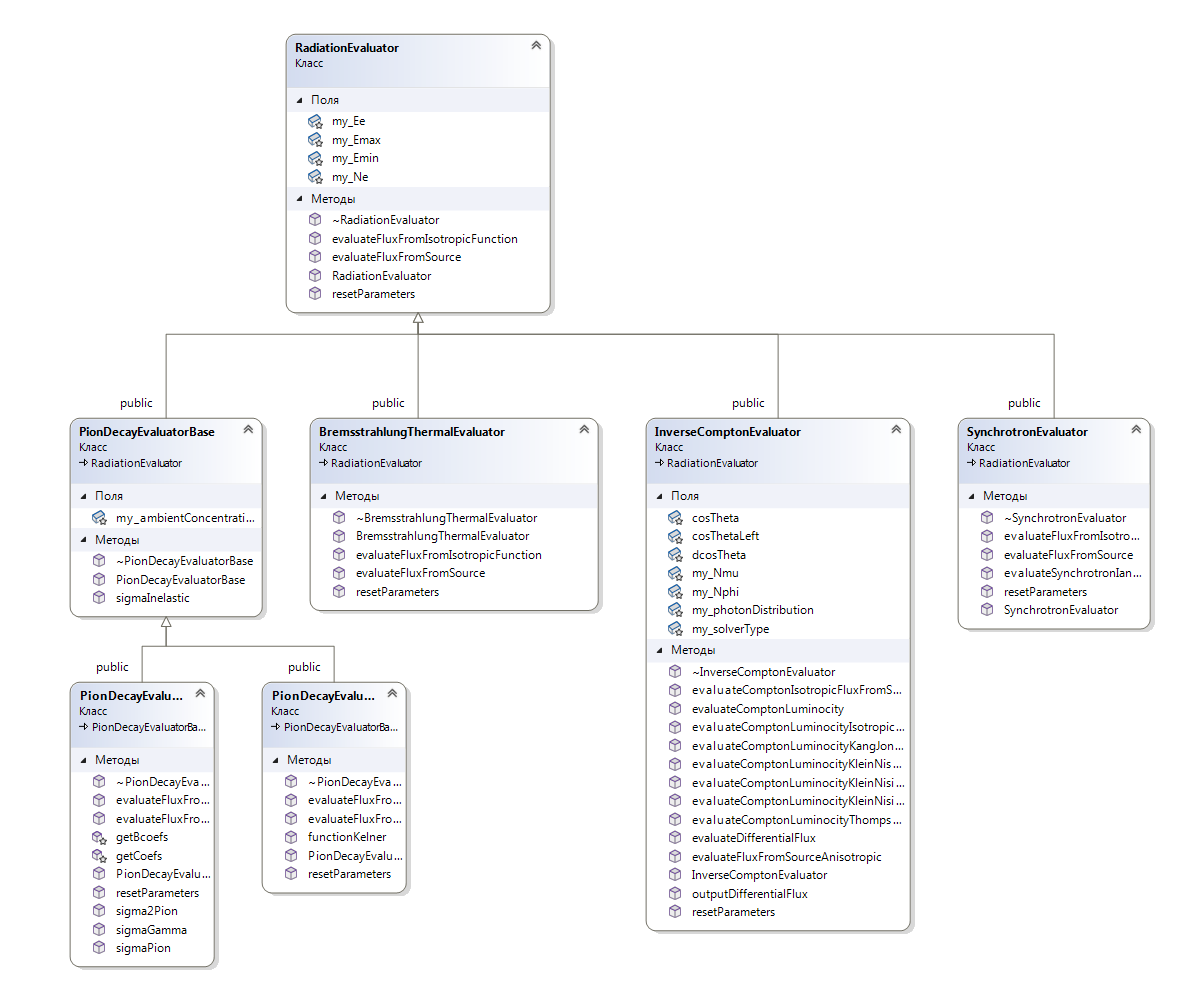
\includegraphics[width=10.5 cm]{./fig/radiationEvaluator.png} 
	\caption{Схема наследования классов вычислителей излучения.}
	\label{radiationEvaluators}
\end{figure}

\subsection{Синхротронное излучение}
Для расчета синхротронного излучения используется класс SynchrotronEvaluator. В нем используется приближение непрерывного спектра, то есть рассматриваемые частоты фотонов предполагаются намного большими, чем частота вращения излучающих частиц в магнитном поле. Реализован случай только изотропной функции распределения излучающих частиц. Так же возможен учет синхротронного самопоглощения. Используемая геометрия источников, показанная на рисунке \ref{sphericalLayer}, позволяет легко интегрировать излучение по лучу зрения, и учитывать при этом поглощение внутри источника. При создании объекта класса необходимо указать рассматриваемый диапазон энергий частиц и количество точек в нем, параметр отвечающий за учет самопоглощения (значение по умолчанию true), а так же значения магнитного поля, синуса угла наклона к лучу зрения и толщины излучаемой области, которые будут использоваться в случае расчета излучения без указания источника, а только с использованием распределения частиц. Публичные методы класса SynchrotronEvaluator перечислены в Таблице \ref{SynchrotronEvaluator}. Пример вычисления синхотронного излучения приведен в разделе \ref{quickStart}.
\begin{table}
	\begin{center}
	\begin{small}
	\caption{Публичные методы классa SynchrotronEvaluator }
	\label{SynchrotronEvaluator}
	\begin{tabularx}{\textwidth}{|X|X|} 
		\hline
		\textbf{SynchrotronEvaluator} & класс предназначенный для вычисления синхротронного излучения\\
		\hline
		SynchrotronEvaluator( int Ne, double Emin, double Emax, bool selfAbsorption = true, bool doppler = false) & конструктор, создает экземпляр с указанным диапазоном рассматриваемых энергий излучающих частиц,и параметрами учета самопоглощения и допплеровского эффекта\\
		\hline
		evaluateSynchrotronIandA(const double\& photonFinalFrequency, const double\& photonFinalTheta, const double\& photonFinalPhi, const double\& B, const double\& sinhi, const double\& concentration, MassiveParticleIsotropicDistribution* electronDistribution, double\& I, double\& A) & вычисляет значения плотности излучательной способности и коэффициента поглощения для фотона с данной энергией и направлением, в области с данными концентрацией и распределением излучающих частиц в данном магнитном поле\\
		\hline
	\end{tabularx}
\end{small}
\end{center}
\end{table}
\subsection{Обратное комптоновское рассеяние}
Для расчета излучения, получающегося в результате процесса обратного комптоновского рассеяния, использеуются классы InverseComptonEvaluator и его наследник InverseComptonEvaluatorWithSource. Отличие между ними в том, что в первом функция распределения рассеиваемых фотонов одинакова во всем излучающем объеме, а во втором изменяется обратно пропорционально квадрату расстояния до источника фотонов. Внутри класса  InverseComptonEvaluator реализованы четыре различных метода расчета излучения, для обозначения которых используется перечислимый тип ComptonSolverType, имеющий следующие значения:

\begin{itemize}
	\item ISOTROPIC\_THOMSON - модель рассеяния в томсоновсков режиме. Реализовано только для степенного распределения электронов и теплового фотонов \cite{Ginzburg1975} глава 17, с. 466
	\item ANISOTROPIC\_KLEIN\_NISHINA - модель расчитывающее излучение напрямую из сечения Клейна-Нишины, возможен учет анизотропных функций распределения \cite{KleinNishina, Dubus}
	\item ISOTROPIC\_KLEIN\_NISHINA - модель расчитывающее излучение напрямую из сечения Клейна-Нишины, но для изотропных функций распределения, что позволяет уменьшить количество интегрирований
	\item ISOTROPIC\_JONES - модель, использующая аналитически проинтегрированное по углам сечение Клейна-Нишины \cite{JonesCompton, BykovUvarov2000}
\end{itemize}

При создании объекта класса InverseComptonEvaluator необходимо указать рассматриваемый диапазон энергий частиц и количество точек в нем, количество ячеек в сетке по полярному и азимутальному углу, изотропную функцию распределения фотонов, которая будет использоваться по умолчанию и метод расчета излучения. Публичные методы классов InverseComptonEvaluator и InverseComptonEvaluatorWithSource перечислены в Таблице \ref{InverseComptonEvaluator}.
\begin{small}
	\topcaption{Публичные методы классa InverseComptonEvaluator }
	\label{InverseComptonEvaluator}
	\begin{xtabular}{|p{0.5\textwidth}|p{0.5\textwidth}|} 
		\hline
		\textbf{InverseComptonEvaluator} & класс предназначенный для вычисления излучения рождащегося в результате обратного комптоновского рассеяния\\
		\hline
		InverseComptonEvaluator( int Ne, int Nmu, int Nphi, double Emin, double Emax, PhotonDistribution* photonDistribution, ComptonSolverType solverType) & конструктор, создает экземпляр с заданным рассматриваемым диапазоном энергии, количеством ячеек в сетке по полярному и азимутальному углу, функцией распределения фотонов, которая будет использоваться по умолчанию и методом расчета излучения\\
		\hline
		evaluateComptonFluxKleinNishinaAnisotropic const double\& photonFinalEnergy, const double\& photonFinalTheta, const double\& photonFinalPhi, PhotonDistribution* photonDistribution, MassiveParticleDistribution* electronDistribution, const double\& volume, const double\& distance) & возвращает энергетическую плотность потока энергии в заданном направлении, излучением созданным заданными функциями распределения фотонов и рассеивющих частиц (которые могут быть анизотропными) в заданном объеме на данном расстоянии\\
		\hline
		evaluateFluxFromSourceAnisotropic( const double\& photonFinalEnergy, const double\& photonFinalTheta, const double\& photonFinalPhi, PhotonDistribution* photonDistribution, RadiationSource* source) & возвращает энергетическую плотность потока энергии в заданном направлении, излучением созданным заданными распределения фотонов и источником, содержащим распределения рассеивающих частиц\\
		\hline
		\textbf{InverseComptonEvaluatorWithSource} & класс предназначенный для вычисления излучения рождащегося в результате обратного комптоновского рассеяния с учетом зависимости функции распределения фотонов от расстояния до их источника\\
		\hline
		InverseComptonEvaluatorWithSource(int Ne, int Nmu, int Nphi, double Emin, double Emax, double Ephmin, double Ephmax, PhotonDistribution* photonDistribution, ComptonSolverType solverType, const double\& sourceR, const double\& sourceZ, const double\& sourcePhi) & конструктор, создает экземпляр с заданным рассматриваемым диапазоном энергии, количеством ячеек в сетке по полярному и азимутальному углу, функцией распределения фотонов, методом расчета излучения и координатами источника фотонов\\
		\hline
	\end{xtabular}
\end{small}

Пример вычисления излучения от обратного комптоновского рассеяние содержится в процедуре evaluateComtonWithPowerLawDistribution() в файле examples.cpp. В ней расчитывается рентгеновское излучение, исходящее от объекта CSS161010 при рассеивании степенного распределения электронов, определенного в работе \cite{Coppejans2020}, на среднегалактическом распределении фотонов.  Сначала определим переменные, задающие основные параметры источника - концентрацию частиц, его размер и магнитное поле. Для вычисления обратного комптоновского рассеяния магнитное поле не используется, но в источнике нужно его задать, поэтому положим его равным нулю. Так же зададим параметры сетки по энергиям и углам, которая будет использоваться вычислителем

\begin{lstlisting}[language=c++]
	double electronConcentration = 150;
	double sinTheta = 1.0;
	double rmax = 1.3E17;
	double B = 0.0;
	double distance = 150*1E6*parsec;
	
	double Emin = me_c2;
	double Emax = 1000 * me_c2;
	int Ne = 200;
	int Nmu = 20;
	int Nphi = 4;
\end{lstlisting}

Далее создадим распределение фотонов, воспользовавшись статическим методом класса MultiPlankDistribution getGalacticField, который возвращает среднегалактическое фотонное распределение, и распределение электронов - возьмем степенное рспределение с показателем 3.5.
\begin{lstlisting}[language=c++]
	PhotonIsotropicDistribution* photonDistribution = 
	    PhotonMultiPlankDistribution::getGalacticField();
	MassiveParticlePowerLawDistribution* electrons = new 
	    MassiveParticlePowerLawDistribution(massElectron, 3.5,
	    Emin, electronConcentration);
\end{lstlisting}

С помощью введенных ранее переменных создадим источник излучения и вычислитель излучения. В качестве метода расчета выберем самый универсальный - ANISOTROPIC\_KLEIN\_NISHINA

\begin{lstlisting}[language=c++]
	RadiationSource* source = new SimpleFlatSource(
	  electrons, B, sinTheta, rmax, rmax, distance);
	
	InverseComptonEvaluator* comptonEvaluator = new 
	    InverseComptonEvaluator(Ne, Nmu, Nphi, Emin, Emax, 
	    photonDistribution, ComptonSolverType::ANISOTROPIC_KLEIN_NISHINA);
\end{lstlisting}

Предположим, что мы не хотим пользоваться встроенным методом вывода излучения в файл, так как хотим получить конечный результат в других единицах, например энергию фотона измерять в электронвольтах, а поток вывести в формате $E F(E)$ - $\text{эрг}\text{см}^{-2}\text{с}^{-1}$. Создадим тогда сетку значений энергии фотонов
\begin{lstlisting}[language=c++]
	int Nnu = 200;
	double* E = new double[Nnu];
	double* F = new double[Nnu];
	double Ephmin = 0.01 * kBoltzman * 2.725;
	double Ephmax = 2 * Emax;
	double factor = pow(Ephmax / Ephmin, 1.0 / (Nnu - 1));
	E[0] = Ephmin;
	F[0] = 0;
	for (int i = 1; i < Nnu; ++i) {
		E[i] = E[i - 1] * factor;
		F[i] = 0;
	}
\end{lstlisting}
после этого вычислим в цикле желаемые потоки излучения
\begin{lstlisting}[language=c++]
	for (int i = 0; i < Nnu; ++i) {
		F[i] = comptonEvaluator->evaluateFluxFromSource(
		    E[i], source);
	}
\end{lstlisting}
и запишем их в файл, переведя в желаемые единицы
\begin{lstlisting}[language=c++]
	FILE* output_ev_EFE = fopen("output.dat", "w");
	
	for (int i = 0; i < Nnu; ++i) {
		double nu = E[i] / hplank;
		fprintf(output_ev_EFE, "%g %g\n",
		    E[i] / (1.6E-12), E[i] * F[i]);
	}

	fclose(output_ev_EFE);
\end{lstlisting}
Спектр излучения, полученный в результате работы данной программы приведен на рисунке \ref{compton}
\begin{figure}
	\centering
	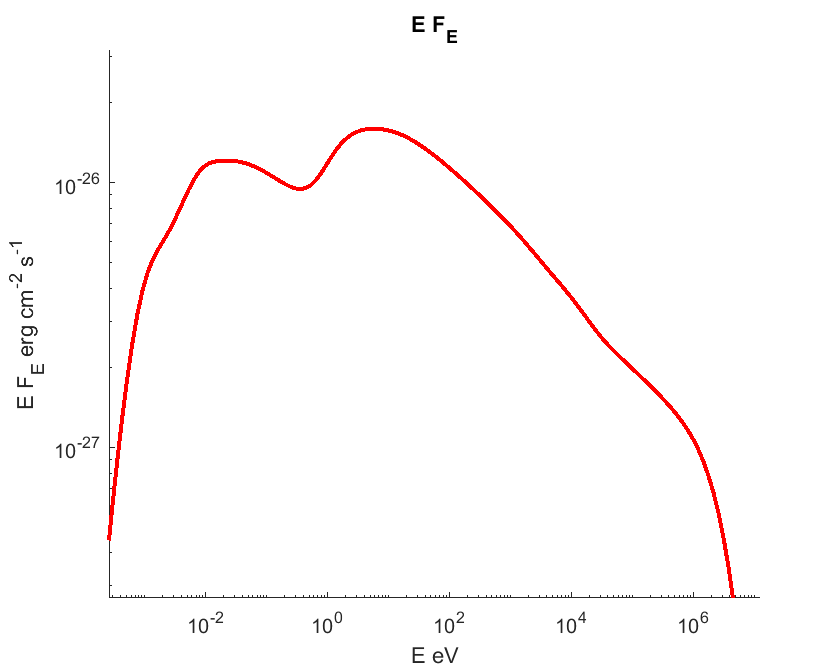
\includegraphics[width=12.5 cm]{./fig/compton.png} 
	\caption{Энергетическая плотность потока синхротронного излучения от тестового источника}
	\label{compton}
\end{figure}

\subsection{Распад пионов}

Для расчета излучения, получающегося в результате распада пионов, родившихся в результате свободно-свободного взаимодействия протонов использеутся абастрактный класс PionDecayEvaluatorBase и двае его наследника: PionDecayEvaluatorKelner, в котором сечение излучения гамма-фотона считается долей от полного сечения неупругого взаимодействия протонов, как описано в статье \cite{Kelner}, и PionDecayEvaluator, в котором используется более точное описание сечения рождения пионов на низких энергиях по методу, описанному в \cite{Kafexhiu}. В текущей версии предполагается, что характерное время потерь энергии протонов при неупругом взаимодействии намного больше времени их удержания в источнике, система является прозрачной для протонов, и каждый из них взаимодействует не более одного раза. В противном случае используемая модель излучения не применима.

При создании объекта класса PionDecayEvaluator необходимо указать рассматриваемый диапазон энергий частиц и количество точек в нем, а так же концентрацию фоновых протонов, так как предполагается рассеяние высокоэнергичных фотонов на покоящихся, а не взаимодействие высокоэнергичных между собой. Публичные методы класса PionDecayEvaluatorBase и его наследников приведены в Таблице \ref{pionDecay}

		\begin{small}
			\topcaption{Публичные методы классa PionDecayEvaluatorBase и его наследников }
			\label{pionDecay}
			\begin{xtabular}{|p{0.5\textwidth}|p{0.5\textwidth}|}  
				\hline
				\textbf{PionDecayEvaluatorBase} & абстрактный класс для вычисления гамма излучения от распада пионов\\
				\hline
				sigmaInelastic(const double\& energy) & возвращает полное сечение неупругого взаимодействия протонов в лабораторной системе, принимает кинетическую энергию движущегося протона\\
				\hline
				\textbf{PionDecayEvaluatorKelner} & класс для вычисления гамма излучения от распада пионов по методу из статьи \cite{Kelner}\\
				\hline
				PionDecayEvaluatorKelner(int Ne, double Emin, double Emax, const double\& ambientConcentration) & конструктор, создает экземпляр с заданным рассматриваемым диапазоном энергии и концентрацией фоновых протонов\\
				\hline
				\textbf{PionDecayEvaluator} & класс для вычисления гамма излучения от распада пионов по методу из статьи \cite{Kafexhiu}\\
				\hline
				PionDecayEvaluator(int Ne, double Emin, double Emax, const double\& ambientConcentration) & конструктор, создает экземпляр с заданным рассматриваемым диапазоном энергии и концентрацией фоновых протонов\\
				\hline
				sigmaGamma(const double\& photonEnergy, const double\& protonEnergy) & возвращает дифференциальное сечение рождения фотона с данной энергией при данной кинетической энергии протона, усредненное по углам\\
				\hline
			\end{xtabular}
		\end{small}

Пример вычисления излучения от гамма излучения от распада пионов показан в функции evaluatePionDecay() в файлк examples.cpp. В нем рассмотрено моделирование излучение объекта Кокон Лебедя в модели ускорения частиц на вторичных ударных волнах, следуя статье \cite{BykovKalyashova2022}. В данной работе вычислено, что спектр ускоренных протонов имеет вид степенной функции с изломом со следующими параметрами - показатели спектра 2.1 и 2.64 на низких и высоких энергиях соответственно, энергия излома - 2.2 ТэВ. Размер излучающей области брался равным размеру сверхкаверны Лебедя - 55 пк. Как и ранее, сначала определим переменные, задающие основные параметры источника - концентрацию частиц, его размер и магнитное поле, которое опять положим равным нулю. Диапазон энергий протонов рассмотрим от 0.01 ГэВ до 10 ТэВ. Так же укажем энергию излома.
\begin{lstlisting}[language=c++]
	double protonConcentration = 150;
	double rmax = 55 * parsec;
	double B = 0;
	double sinTheta = 1.0;

	double distance = 1400 * parsec;
	double Emin = massProton*speed_of_light2 + 0.01E9 * 1.6E-12;
	double Emax = 1E13 * 1.6E-12;
	double Etrans = 2.2E12 * 1.6E-12;
\end{lstlisting}
После этого создадим распределение протонов и источник излучения
\begin{lstlisting}[language=c++]
	MassiveParticleBrokenPowerLawDistribution* protons = new 
		MassiveParticleBrokenPowerLawDistribution(
		massProton, 2.1, 2.64, Emin, Etrans, protonConcentration);
	RadiationSource* source = new SimpleFlatSource(
		protons, B, sinTheta, rmax, rmax, distance);
\end{lstlisting}
Далее потребуется вычислитель излучения. В случае пионного распада необходимо указать концентрацию фоновых протонов.
\begin{lstlisting}[language=c++]
double protonAmbientConcentration = 20;
PionDecayEvaluator* pionDecayEvaluator = new PionDecayEvaluator(
	200, Emin, Emax, protonAmbientConcentration);
\end{lstlisting}
Как и в предыдущих случаях далее необходимо внутри цикла вычислить излучение в интересующем диапазоне энергий, используя функцию evaluateFluxFromSource, и вывести результат в файл в удобных единицах. Спектр излучения, полученный в результате работы данной программы и результаты наблюдений Кокона Лебедя на Fermi LAT, ARGO и HAWC \cite{Ackermann2011, Bartoli2014, Abeysekara2021} приведены на рисунке \ref{pion}
\begin{figure}
	\centering
	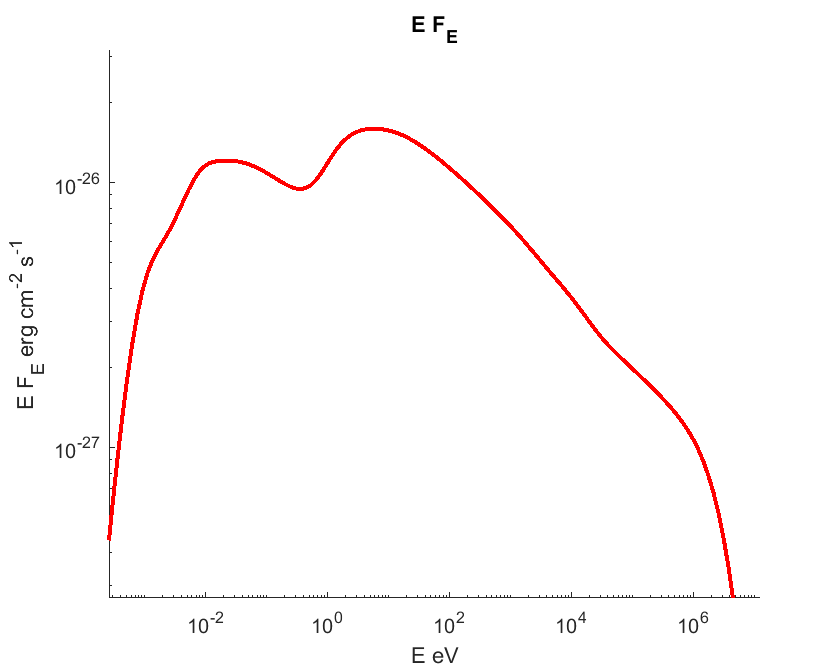
\includegraphics[width=12.5 cm]{./fig/compton.png} 
	\caption{Расчетная энергетическая плотность потока гамма излучения Кокона Лебедя и данные наблюдений}
	\label{pion}
\end{figure}
\subsection{Тормозное излучение}
В текущей версии кода реализовано вычисление тормозного излучения электронов в плазме только для случая теплового распределения. Для этого предназначен класс BremsstrahlungThermalEvaluator. В процессе расчета предполагается, что плазма электрон-протонная, с одинаковыми температурами электронов и протонов, в вычислении используются Гаунт-факторы, приведенные в \cite{Rybicki}. Пример вычисления тормохного излучения приведен в функции evaluateBremsstrahlung в файле examples.cpp.

			% Глава 1. Расчет излучения источников
	\chapter{Evaluation of radiation}\label{evaluation}
In current version of the code following types of radiation are implemented: synchrotron radiation, inverse Compton scattering, gamma-ray emission due to pion decay in free-free proton interaction and also bremsstrahlung.

Abstract class RadiationEvaluator and it's inherited classes are used for evaluation of radiation. There are derved classes for every specific type of radiation and also class RadiationSumEvaluator which allows to sum several different types of radiation. Public methods of this two classes are listed in Table \ref{radiationEvaluator}. 

General approach to evaluation of radiation is following: create radiation source, using one of the classes, described in Section \ref{sourcesSection}, or user-defined, then create object of radiation evaluator, which types are described below, and then call method evaluateFluxFromSource(const double\& photonFinalEnergy, RadiationSource* source) of this object, which evaluates energy density of the energy flux from source in units $\rm cm^{-2} s^{-1}$.

\begin{figure}[h]
	\centering
	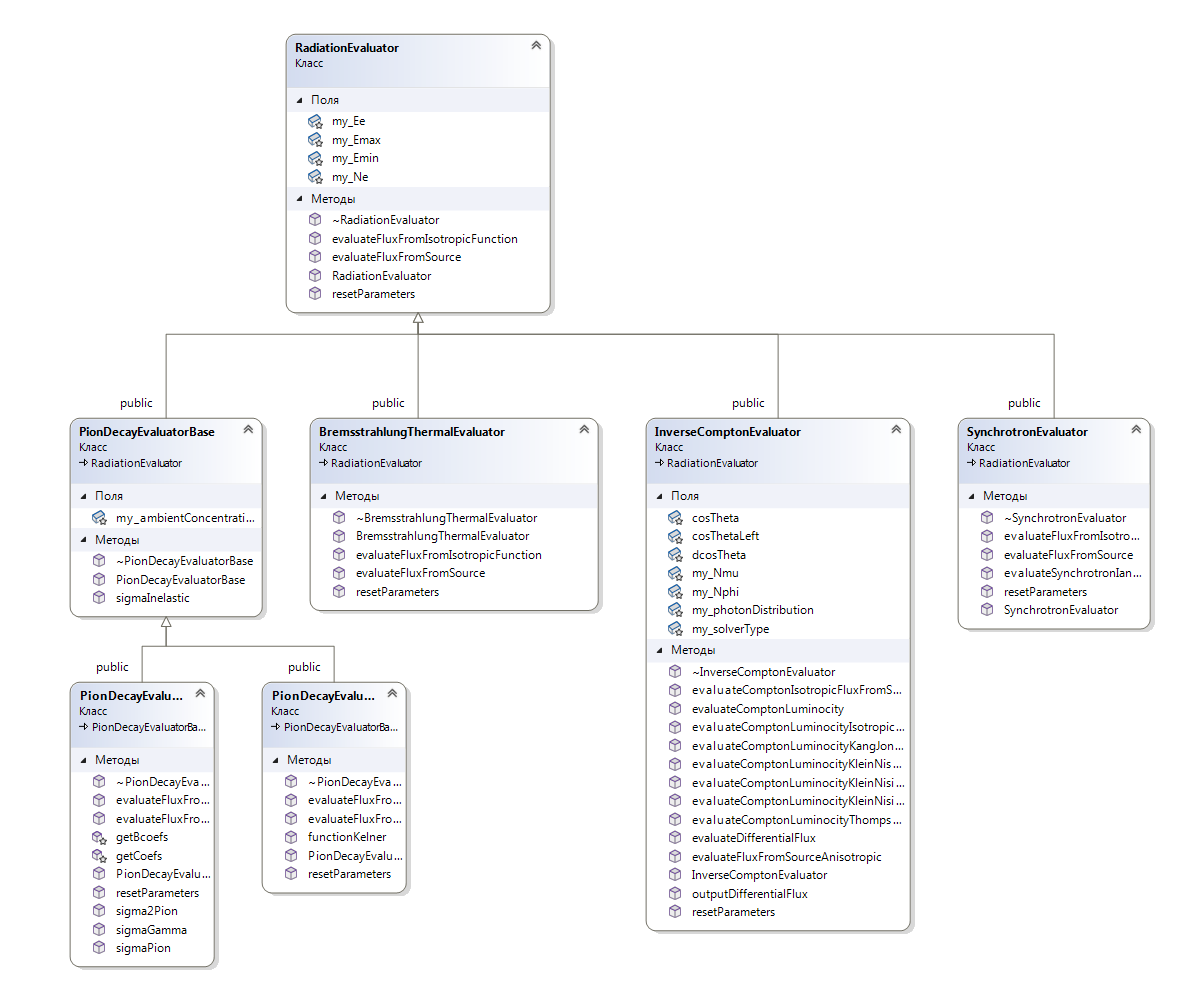
\includegraphics[width=10.5 cm]{./fig/radiationEvaluator.png} 
	\caption{class hierarchy of radiation evaluators}
	\label{radiationEvaluators}
\end{figure}

Classes for every specific type of electromagnetic radiation are described below in this chapter. Class hierarchy of radiation evaluators is shown in Figure \ref{radiationEvaluators}. Equations used for evaluation are discussed in Chapter \ref{Formulae}.

\begin{small}
	\topcaption{Public methods of RadiationEvaluator class}
	\label{radiationEvaluator}
	\begin{xtabular}{|p{0.51\textwidth}|p{0.49\textwidth}|} 
		\hline
		\textbf{RadiationEvaluator} & astract class for evaluation of radiation \\
		\hline
		virtual evaluateFluxFromSource(const double\& photonFinalEnergy, RadiationSource* source) & virtual method, returns energy density of radiation energy flux in units $\text{cm}^{-2} \text{s}^{-1}$ \\
		\hline
		virtual double evaluateFluxFromSourceAtPoint(const double\& photonFinalEnergy, RadiationSource* source, int rhoi, int phi) & virtual method, returns energy density of radiatio energy flux from given grid cell on tangent plane\\
		\hline
		double evaluateTotalFluxInEnergyRange(const double\& Ephmin, const double\& Ephmax, int Nph, RadiationSource* source) & returns integrated energy flux in the given energy range, evaluted by Nph points distributied logarithmically, in units $\text{erg} \text{cm}^{-2} \text{s}^{-1}$\\
		\hline
		virtual resetParameters( const double* parameters, const double* normalizationUnits) & virtual method, reseting parameters of the radiation evaluator. Lists of parameters are different for different types of evaluators. Method takes for input array of parameters in normalized units, and array of normalization conctants. This method for example is used for fitting modelled radiation to the observational data and optimization.\\
		\hline
		writeFluxFromSourceToFile(const char* fileName, RadiationSource* source, const double\& Ephmin, const double\& Ephmax, const int Nph) & evaluates and writes into the file energy density of radiation energy flux in given energy range with Nph points distributed logarithmically. Writes two columns of data in units $\text{erg}$  and $\text{cm}^{-2} \text{s}^{-1}$\\
		\hline
		writeImageFromSourceToFile(const char* fileName, RadiationSource* source, const double\& Ephmin, const double\& Ephmax, const int Nph) & evaluates and writes to file image - energy flux from every cell of the tangent plane in units $\text{erg} \text{cm}^{-2} \text{s}^{-1}$ integrated in given energy range with Nph points distributed logarithmically\\
		\hline
		writeImageFromSourceAtEToFile(const double\& photonFinalEnergy, const char* fileName, RadiationSource* source) & evaluates and writes to file image - energy density of radiation energy flux from every cell of the tangent plane in units $\text{cm}^{-2} \text{s}^{-1}$\\
		\hline
		\textbf{RadiationSumEvaluator} & class for sum of several types of radiation\\
		\hline
		RadiationSumEvaluator(int Ne, const double\& Emin, const double\& Emax, RadiationEvaluator* evaluator1, RadiationEvaluator* evaluator2) & constructor, creates evaluator which sums results of two given evaluators, and takes into accaunt emmiting particles in given energy range\\
		\hline
		RadiationSumEvaluator(int Ne, const double\& Emin, const double\& Emax, int Nev, RadiationEvaluator** evaluators) & constructor, creates evaluator which sums results of given array of evaluators, and takes into accaunt emmiting particles in given energy range\\
		\hline
	\end{xtabular}
\end{small}

\section{Synchrotron radiation}\label{synchrotronSection}
Class SynchrotronEvaluator is implemented for evaluation of synchrotron radiation. It uses standard approximation of continious spectrum, described in \cite{Ginzburg1975, Ghisellini} and in section \ref{synchrotronFormulaSection},  - it is valid for frequencies of emitted photons much higher than gyrofrequency of emitting particles. Also it is possible to take into account synchrotron self-absorption. Cylindrical geomtry, shown in Figure \ref{sphericalLayer} allows to integrate flux through the line of sight and take into account absorption inside the source. To create SynchrotronEvaluator object user should provide energy range of particles to be taken into account, numbers of integration points in it, and also two boolean parameters - for accounting self absorption and doppler shifting due to source matter velocity. Public methods of Synchrotron evaluator are listed in Table  \ref{SynchrotronEvaluator}. Example of evaliation of synchrotron radiation is shown in section \ref{quickStart}.
\begin{table}[h]
	\begin{center}
	\begin{small}
	\caption{Public methods of SynchrotronEvaluator}
	\label{SynchrotronEvaluator}
	\begin{tabularx}{\textwidth}{|X|X|} 
		\hline
		\textbf{SynchrotronEvaluator} & class for evaluation synchrotron radiation\\
		\hline
		SynchrotronEvaluator( int Ne, double Emin, double Emax, bool selfAbsorption = true, bool doppler = false) & constructor, creates evaluator with given energy range of particles taken into account and parameters corresponding to self-absorption and doppler effect\\
		\hline
		evaluateSynchrotronIandA(const double\& photonFinalFrequency, const double\& photonFinalTheta, const double\& photonFinalPhi, const double\& B, const double\& sinhi, const double\& concentration, MassiveParticleIsotropicDistribution* electronDistribution, double\& I, double\& A) & evaluates emissivity per unit volume and absorption coefficient for photon of given energy and direction in given magnetic field and number density and distribution of emitting particles\\
		\hline
	\end{tabularx}
\end{small}
\end{center}
\end{table}
\section{Inverse Compton scattering}
Class InverseComptonEvaluator is implemented for evaluation of radiation produced in inverce compton scattering. Also it has one derived class InverseComptonEvaluatorWithSource. The difference between them is that in the first one distribution of seed photons is constant inside the source, and in the second one photons number density is change proportionaly inverse square of the distance to the source of seed photons.

There are four different algorithmes of evaluation IC radiation that can be used by InverseComptonEvaluator. They are listed by enum-type ComptonSolverType, having following values:

\begin{itemize}
	\item ISOTROPIC\_THOMSON - simple model of scattering in thomson regime with power-law distribution of electrons and thermal distribution of seed photons, as described in \cite{Ginzburg1975} ch 17, p. 466.
	\item ANISOTROPIC\_KLEIN\_NISHINA - model computing radiation directly by integrating Klein-Nishina cros-section as described in \cite{KleinNishina, Dubus} and in section \ref{comptonFormulaSection}. With this model is possible to evaluate radiation produced by anisotropic distributions of initial particles
	\item ISOTROPIC\_KLEIN\_NISHINA - model similar to the previous, it uses integration of Klein-Nishina cross-section, but isotropy of distributions of initial particles is assumed, and it allows to reduce number of integrations through the azimuthal angle
	\item ISOTROPIC\_JONES - model, using analytical integration through the all angular variables, in case of isotropic distributions of initial particles. It is described in \cite{JonesCompton, BykovUvarov2000} and in section??
\end{itemize}

To create object of InverseComptobEvaluator type user needs to provide energy range of particles taken into account and nimber of points to integrate through it, number of points through the polar and azimutal angle, distribution function of seed photons and algorithm of computation the radiation. Public methods of InverseComptonEvaluator and InverseComptonEvaluatorWithSource are listed in Table \ref{InverseComptonEvaluator}.
\begin{small}
	\topcaption{Public methods of inverse compton scattering evaluators}
	\label{InverseComptonEvaluator}
	\begin{xtabular}{|p{0.5\textwidth}|p{0.5\textwidth}|} 
		\hline
		\textbf{InverseComptonEvaluator} & class for evaluation radiation from inverse compton scattering\\
		\hline
		InverseComptonEvaluator( int Ne, int Nmu, int Nphi, double Emin, double Emax, PhotonDistribution* photonDistribution, ComptonSolverType solverType) & constructor, creates evaluator with given energy range of particles taken into account, numbers of integration points throught the energy and angular variables, distribution function of seed photons and method of computation the radiation\\
		\hline
		evaluateFluxFromSourceAnisotropic( const double\& photonFinalEnergy, const double\& photonFinalTheta, const double\& photonFinalPhi, PhotonDistribution* photonDistribution, RadiationSource* source) & returns energy density of radiation energy flux created by given seed photons distribution and source containing scattering particles in given direction\\
		\hline
		evaluateTotalFluxInEnergyRangeAnisotropic( const double\& Ephmin, const double\& Ephmax, const double\& photonFinalTheta, const double\& photonFinalPhi, int Nph, PhotonDistribution* photonDistribution, RadiationSource* source, ComptonSolverType solverType) & returns total energy flux of radiation created by given seed photons distribution and source containing scattering particles in given direction integrated in given energy range through Nph point distributed logarithmically.\\
		\hline
		\textbf{InverseComptonEvaluatorWithSource} & class for evaluation radiation from inverce comton scattering takin into account dependency of photons number density on distance to the source of photons\\
		\hline
		InverseComptonEvaluatorWithSource(int Ne, int Nmu, int Nphi, double Emin, double Emax, double Ephmin, double Ephmax, PhotonDistribution* photonDistribution, ComptonSolverType solverType, const double\& sourceR, const double\& sourceZ, const double\& sourcePhi) & constructor, creates evaluator with given energy range of particles taken into account, numbers of integration points throught the energy and angular variables, distribution function of seed photons with number density corresponding to the origin of coordinates, method of computation the radiation and coordinates of the source of seed photons\\
		\hline
	\end{xtabular}
\end{small}

Пример вычисления излучения от обратного комптоновского рассеяние содержится в процедуре evaluateComtonWithPowerLawDistribution() в файле examples.cpp. В ней расчитывается рентгеновское излучение, исходящее от объекта CSS161010 при рассеивании степенного распределения электронов, определенного в работе \cite{Coppejans2020}, на среднегалактическом распределении фотонов.  Сначала определим переменные, задающие основные параметры источника - концентрацию частиц, его размер и магнитное поле. Для вычисления обратного комптоновского рассеяния магнитное поле не используется, но в источнике нужно его задать, поэтому положим его равным нулю. Так же зададим параметры сетки по энергиям и углам, которая будет использоваться вычислителем

\begin{lstlisting}[language=c++]
	double electronConcentration = 150;
	double sinTheta = 1.0;
	double rmax = 1.3E17;
	double B = 0.0;
	double distance = 150*1E6*parsec;
	
	double Emin = me_c2;
	double Emax = 1000 * me_c2;
	int Ne = 200;
	int Nmu = 20;
	int Nphi = 4;
\end{lstlisting}

Далее создадим распределение фотонов, воспользовавшись статическим методом класса MultiPlankDistribution getGalacticField, который возвращает среднегалактическое фотонное распределение, и распределение электронов - возьмем степенное рспределение с показателем 3.5.
\begin{lstlisting}[language=c++]
	PhotonIsotropicDistribution* photonDistribution = 
	    PhotonMultiPlankDistribution::getGalacticField();
	MassiveParticlePowerLawDistribution* electrons = new 
	    MassiveParticlePowerLawDistribution(massElectron, 3.5,
	    Emin, electronConcentration);
\end{lstlisting}

С помощью введенных ранее переменных создадим источник излучения и вычислитель излучения. В качестве метода расчета выберем самый универсальный - ANISOTROPIC\_KLEIN\_NISHINA

\begin{lstlisting}[language=c++]
	RadiationSource* source = new SimpleFlatSource(
	  electrons, B, sinTheta, rmax, rmax, distance);
	
	InverseComptonEvaluator* comptonEvaluator = new 
	    InverseComptonEvaluator(Ne, Nmu, Nphi, Emin, Emax, 
	    photonDistribution, ComptonSolverType::ANISOTROPIC_KLEIN_NISHINA);
\end{lstlisting}

Предположим, что мы не хотим пользоваться встроенным методом вывода излучения в файл, так как хотим получить конечный результат в других единицах, например энергию фотона измерять в электронвольтах, а поток вывести в формате $E F(E)$ - $\text{эрг}\text{см}^{-2}\text{с}^{-1}$. Создадим тогда сетку значений энергии фотонов
\begin{lstlisting}[language=c++]
	int Nnu = 200;
	double* E = new double[Nnu];
	double* F = new double[Nnu];
	double Ephmin = 0.01 * kBoltzman * 2.725;
	double Ephmax = 2 * Emax;
	double factor = pow(Ephmax / Ephmin, 1.0 / (Nnu - 1));
	E[0] = Ephmin;
	F[0] = 0;
	for (int i = 1; i < Nnu; ++i) {
		E[i] = E[i - 1] * factor;
		F[i] = 0;
	}
\end{lstlisting}
после этого вычислим в цикле желаемые потоки излучения
\begin{lstlisting}[language=c++]
	for (int i = 0; i < Nnu; ++i) {
		F[i] = comptonEvaluator->evaluateFluxFromSource(
		    E[i], source);
	}
\end{lstlisting}
и запишем их в файл, переведя в желаемые единицы
\begin{lstlisting}[language=c++]
	FILE* output_ev_EFE = fopen("output.dat", "w");
	
	for (int i = 0; i < Nnu; ++i) {
		double nu = E[i] / hplank;
		fprintf(output_ev_EFE, "%g %g\n",
		    E[i] / (1.6E-12), E[i] * F[i]);
	}

	fclose(output_ev_EFE);
\end{lstlisting}
Спектр излучения, полученный в результате работы данной программы приведен на рисунке \ref{compton}
\begin{figure}
	\centering
	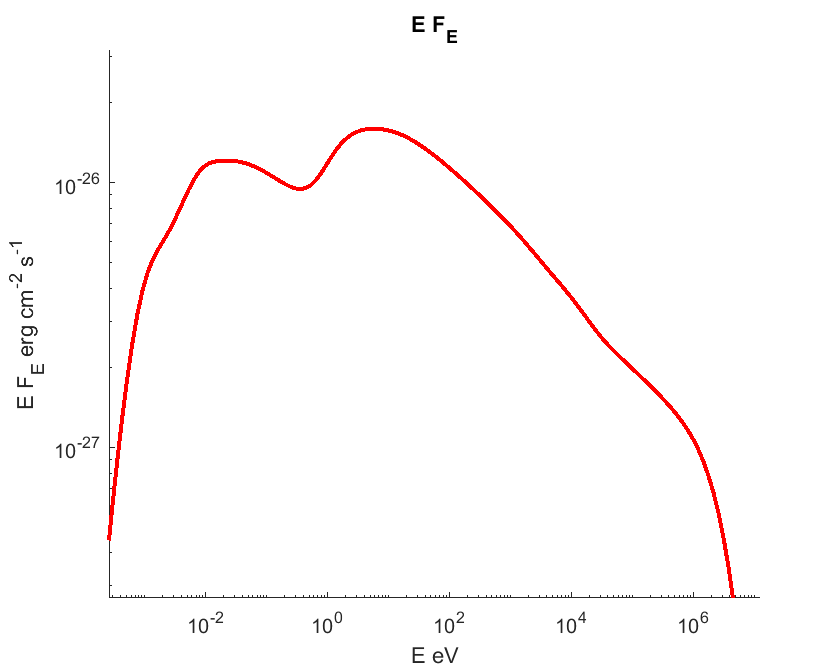
\includegraphics[width=12.5 cm]{./fig/compton.png} 
	\caption{Энергетическая плотность потока синхротронного излучения от тестового источника}
	\label{compton}
\end{figure}

\section{Распад пионов}

Для расчета излучения, получающегося в результате распада пионов, родившихся в результате свободно-свободного взаимодействия протонов использеутся абастрактный класс PionDecayEvaluatorBase и двае его наследника: PionDecayEvaluatorKelner, в котором сечение излучения гамма-фотона считается долей от полного сечения неупругого взаимодействия протонов, как описано в статье \cite{Kelner}, и PionDecayEvaluator, в котором используется более точное описание сечения рождения пионов на низких энергиях по методу, описанному в \cite{Kafexhiu}. В текущей версии предполагается, что характерное время потерь энергии протонов при неупругом взаимодействии намного больше времени их удержания в источнике, система является прозрачной для протонов, и каждый из них взаимодействует не более одного раза. В противном случае используемая модель излучения не применима.

При создании объекта класса PionDecayEvaluator необходимо указать рассматриваемый диапазон энергий частиц и количество точек в нем, а так же концентрацию фоновых протонов, так как предполагается рассеяние высокоэнергичных фотонов на покоящихся, а не взаимодействие высокоэнергичных между собой. Публичные методы класса PionDecayEvaluatorBase и его наследников приведены в Таблице \ref{pionDecay}

		\begin{small}
			\topcaption{Публичные методы классa PionDecayEvaluatorBase и его наследников }
			\label{pionDecay}
			\begin{xtabular}{|p{0.5\textwidth}|p{0.5\textwidth}|}  
				\hline
				\textbf{PionDecayEvaluatorBase} & абстрактный класс для вычисления гамма излучения от распада пионов\\
				\hline
				sigmaInelastic(const double\& energy) & возвращает полное сечение неупругого взаимодействия протонов в лабораторной системе, принимает кинетическую энергию движущегося протона\\
				\hline
				\textbf{PionDecayEvaluatorKelner} & класс для вычисления гамма излучения от распада пионов по методу из статьи \cite{Kelner}\\
				\hline
				PionDecayEvaluatorKelner(int Ne, double Emin, double Emax, const double\& ambientConcentration) & конструктор, создает экземпляр с заданным рассматриваемым диапазоном энергии и концентрацией фоновых протонов\\
				\hline
				\textbf{PionDecayEvaluator} & класс для вычисления гамма излучения от распада пионов по методу из статьи \cite{Kafexhiu}\\
				\hline
				PionDecayEvaluator(int Ne, double Emin, double Emax, const double\& ambientConcentration) & конструктор, создает экземпляр с заданным рассматриваемым диапазоном энергии и концентрацией фоновых протонов\\
				\hline
				sigmaGamma(const double\& photonEnergy, const double\& protonEnergy) & возвращает дифференциальное сечение рождения фотона с данной энергией при данной кинетической энергии протона, усредненное по углам\\
				\hline
			\end{xtabular}
		\end{small}

Пример вычисления излучения от гамма излучения от распада пионов показан в функции evaluatePionDecay() в файлк examples.cpp. В нем рассмотрено моделирование излучение объекта Кокон Лебедя в модели ускорения частиц на вторичных ударных волнах, следуя статье \cite{BykovKalyashova2022}. В данной работе вычислено, что спектр ускоренных протонов имеет вид степенной функции с изломом со следующими параметрами - показатели спектра 2.1 и 2.64 на низких и высоких энергиях соответственно, энергия излома - 2.2 ТэВ. Размер излучающей области брался равным размеру сверхкаверны Лебедя - 55 пк. Как и ранее, сначала определим переменные, задающие основные параметры источника - концентрацию частиц, его размер и магнитное поле, которое опять положим равным нулю. Диапазон энергий протонов рассмотрим от 0.01 ГэВ до 10 ТэВ. Так же укажем энергию излома.
\begin{lstlisting}[language=c++]
	double protonConcentration = 150;
	double rmax = 55 * parsec;
	double B = 0;
	double sinTheta = 1.0;

	double distance = 1400 * parsec;
	double Emin = massProton*speed_of_light2 + 0.01E9 * 1.6E-12;
	double Emax = 1E13 * 1.6E-12;
	double Etrans = 2.2E12 * 1.6E-12;
\end{lstlisting}
После этого создадим распределение протонов и источник излучения
\begin{lstlisting}[language=c++]
	MassiveParticleBrokenPowerLawDistribution* protons = new 
		MassiveParticleBrokenPowerLawDistribution(
		massProton, 2.1, 2.64, Emin, Etrans, protonConcentration);
	RadiationSource* source = new SimpleFlatSource(
		protons, B, sinTheta, rmax, rmax, distance);
\end{lstlisting}
Далее потребуется вычислитель излучения. В случае пионного распада необходимо указать концентрацию фоновых протонов.
\begin{lstlisting}[language=c++]
double protonAmbientConcentration = 20;
PionDecayEvaluator* pionDecayEvaluator = new PionDecayEvaluator(
	200, Emin, Emax, protonAmbientConcentration);
\end{lstlisting}
Как и в предыдущих случаях далее необходимо внутри цикла вычислить излучение в интересующем диапазоне энергий, используя функцию evaluateFluxFromSource, и вывести результат в файл в удобных единицах. Спектр излучения, полученный в результате работы данной программы и результаты наблюдений Кокона Лебедя на Fermi LAT, ARGO и HAWC \cite{Ackermann2011, Bartoli2014, Abeysekara2021} приведены на рисунке \ref{pion}
\begin{figure}
	\centering
	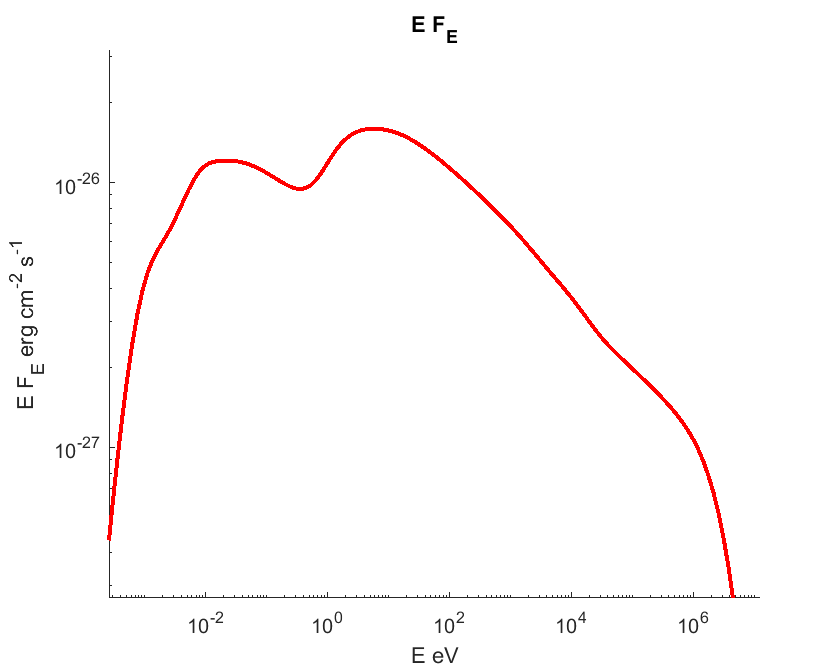
\includegraphics[width=12.5 cm]{./fig/compton.png} 
	\caption{Расчетная энергетическая плотность потока гамма излучения Кокона Лебедя и данные наблюдений}
	\label{pion}
\end{figure}
\section{Тормозное излучение}
В текущей версии кода реализовано вычисление тормозного излучения электронов в плазме только для случая теплового распределения. Для этого предназначен класс BremsstrahlungThermalEvaluator. В процессе расчета предполагается, что плазма электрон-протонная, с одинаковыми температурами электронов и протонов, в вычислении используются Гаунт-факторы, приведенные в \cite{Rybicki}. Пример вычисления тормохного излучения приведен в функции evaluateBremsstrahlung в файле examples.cpp.

			% Глава 2. Оптимизация параметров
	\chapter{Parameters optimization}\label{optimization}
Code FAINA allows not only to evaluate radiation from the source, but also to fit model data to observations and obtain parameters of the source. There are various types optimization methods and models of loss functions, implemented in the code.

\section{Evaluators of the loss function}

The first thing one should determine to start optimization process is a loss function. In FAINA code abstract class LossEvalator and derived classes are used for it. All implemented classes use quadratic loss functions, taking into account observational errors:
$L = \sum \frac{(F_i - F_{obs,i})^2}{\sigma_i^2}$, where $F_i$ - is some modeled function of radiation (e.g. energy spectral density) evaluated at point corresponding to some observation, $F_{obs,i}$ - observed value of this function, $\sigma_i$ - it's uncertainty. There are following classes of loss function evaluator implemented in the code: SpectrumLossEvaluator - for fitting energy flux spectral density at given time moment, TimeDependentSpectrumLossEvaluator - for fitting energy flux spectral density in different time moments and RadialProfileLossEvaluator - for fitting luminosity of the prolonged source in different points depending on coordinate in tangent plane. Public methods of this classes are listed in Table \ref{LossEvaluators}.

\begin{small}
	\topcaption{Public methods of loss function evaluators}
	\label{LossEvaluators}
	\begin{xtabular}{|p{0.5\textwidth}|p{0.5\textwidth}|}
		\hline
		\textbf{LossEvaluator} & abstract class for evaluator of loss function\\
		\hline
		virtual double evaluate(const double* vector, const double* maxParameters, RadiationEvaluator* evaluator) & virtual method, returns value of loss function with given parameters. Also takes vector of normalization units for parameters and radiation evaluator\\
		\hline
		\textbf{SpectrumLossEvaluator} & class for fitting energy flux energy density. Loss function is $L = \sum \frac{(F(E_i) - F_{obs,i})^2}{\sigma_i^2}$, where $F(E_i)$ - modeled energy flux energy density evaluated at energy $E_i$, $F_{obs,i}$ - corresponding observed value, $\sigma_i$ - it's uncertancy.\\
		\hline
		SpectrumLossEvaluator(double* energy, double* observedFlux, double* observedError, int Ne, RadiationSource* radiatiornSource) & constructor, creates loss evaluator, with given values of energies of observational points, observed fluxes and it's uncertancies, number of points and radiation source\\
		\hline
		\textbf{TimeDependentSpectrumLossEvaluator} & class fitting energy flux energy density at different time moments. Loss function is $L = \sum \frac{(F(E_{ij}, t_j) - F_{obs,i,j})^2}{\sigma_{ij}^2}$, where $F(E_{ij},t_j)$ - modeled energy flux energy density evaluated at energy $E_{ij}$ at time moment $t_j$, $F_{obs,i,j}$ - corresponding observed value, $\sigma_{ij}$ - it's uncertancies. NOTE that number of energy grid point may be different at different time moments\\
		\hline
		TimeDependentSpectrumLossEvaluator(double** energy, double** observedFlux, double** observedError, int* Ne, double* times, int Ntimes, RadiationTimeDependentSource* radiationSource) & constructor, creates loss evaluator with given values of energies of observational points, observed fluxes and it's uncertancies, numbers of energy grid points, time moments, number of time grid points and radiation source\\
		\hline
		\textbf{RadialProfileLossEvaluator} & class for fitting luminocity of different points of the source, depending of radius in tangent plane. Loss function is $L = \sum \frac{(F(R_i) - F_{obs,i})^2}{\sigma_i^2}$, where $F(R_i)$ - energy flux surface density, at given radius $R_i$, $F_{obs,i}$ - corresponding observed value, $\sigma_i$ - it's uncertancy\\
		\hline
		RadialProfileLossEvaluator(double energy, double* observedFlux, double* observedError, double* rhoPoints, int Nrho, RadiationSource* radiaionSource) & constructor, creates loss evaluator, wuth given value of energy to evaluate flux density, observed value of luminocity surface density, observed value and it's uncertancies, radius grid points, number of grid points and radiation source\\
		\hline
	\end{xtabular}
\end{small}

\section{Optimizers of loss function}

For fitting modeled radiation from the source to observational data, abstract class RadiationOptimizer is implemented. It has virtual function optimize(double* vector, bool* optPar) which performs minimization of loss function. This function takes as input array of parameters of the source vector, and boolean array optPar showing for each parameter to optimize it or consider it fixed. Array of parameters must be consistent with function of used radiation source resetParameters, which was described in section \ref{sourcesSection}, because this function will be used during optimization and take the same array of parameters as input.

There are three implemented classes, inherited from RadiationOptimizer: GridEnumRadiationOptimizer, which finds minimum of loss function on the fixed logarithmic grid in the parameters space, GradientDescentRadiationOptimizer, which uses gradient descent method and CombinedRadiationOptimizer, and sequentially applies these methods, using result of search on the grid as starting point for gradient descent. Hierarchy scheme of optimizers classes is shown in Figure \ref{radiationOptimizer}, and public methods are listed in Table \ref{RadiationOptimizerMethods}. Implemented optimization methods can be applied to any types of sources, electro-magnetic radiation and loss function evaluators which were described above.
\begin{figure}
	\centering
	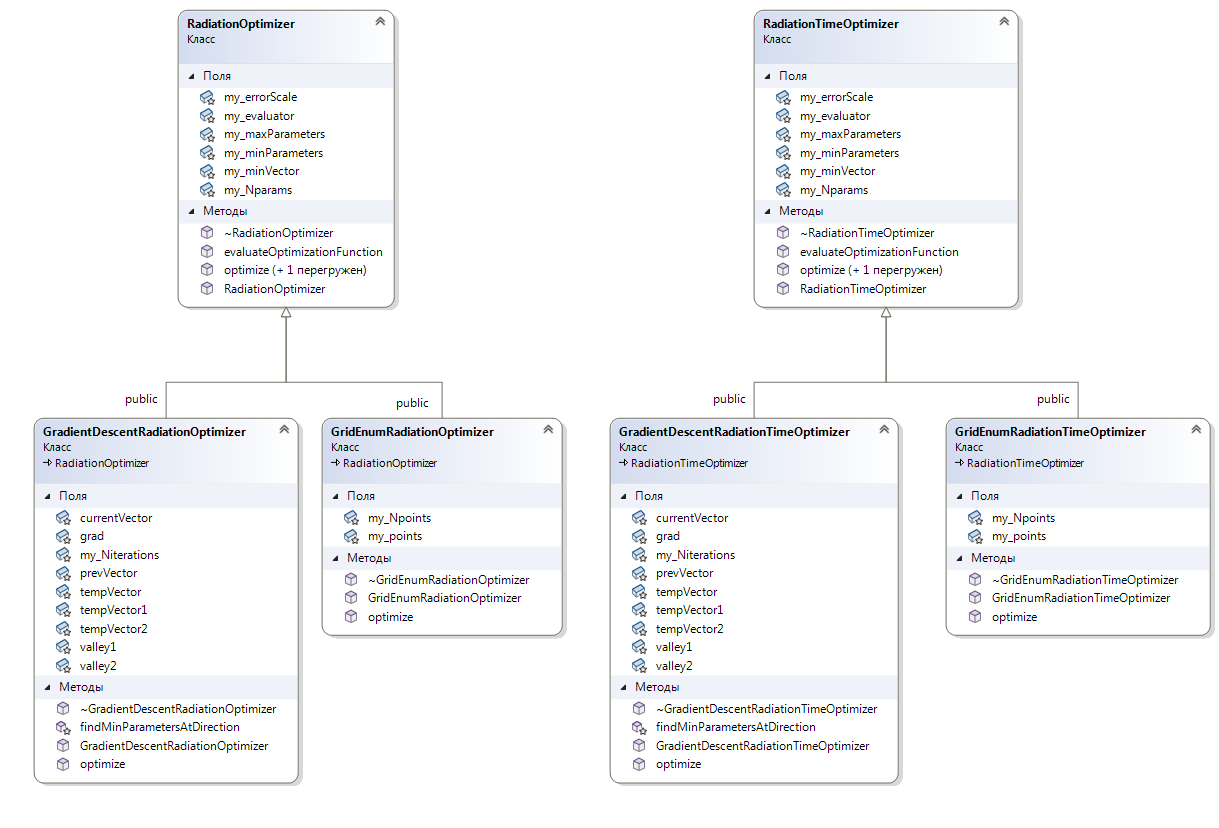
\includegraphics[width=11.5 cm]{./fig/radiationOptimizer.png} 
	\caption{class hierarchy of radiation optimizers}
	\label{radiationOptimizer}
\end{figure}

\begin{small}
	\topcaption{Public methods of radiation optimizer classes}
	\label{RadiationOptimizerMethods}
	\begin{xtabular}{|p{0.41\textwidth}|p{0.59\textwidth}|}
		\hline
		\textbf{RadiationOptimizer} & abstract class for fitting modeled radiation to observations and optimization of source parameters \\
		\hline
		double evaluateOptimizationFunction( const double* vector) & returns value of loss function with given parameters\\
		\hline
		void optimize( double* vector, bool* optPar) & performs optimization, takes array of peremeters, where final values would be writen, and array of boolean values showing to optimize corresponding parameter or consider it fixed \\
		\hline
		void outputProfileDiagrams( const double* vector, int Npoints) & evaluates and writes into files 2d profiles of loss function in parameters space which contain starting point, defined by array vector, for all possible pairs of parameters\\
		\hline
		void outputOptimizedProfileDiagram( const double* vector, bool* optPar, int Npoints, int Nparam1, int Nparam2) & evaluates and writes into file 2d profile of loss function in plane in the parameter space, defined by parameter numbers Nparam1 and Nparam2, containing starting point in it, with given nuber of grid points for this parameters, while other parameters are optimized, if it is allowed by boolean array optPar\\
		\hline
		\textbf{GridEnumRadiationOptimizer} & class for optimization by search of minimum value on the fixed logarithmic grid in parameters space\\
		\hline
		GridEnumRadiationOptimizer( RadiationEvaluator* evaluator, const double* minParameters, const double* maxParameters, int Nparams, const int* Npoints, LossEvaluator* lossEvaluator) & constructor, creates optimizer with given radiation evaluator, domain of parameters defined by minimum and maximum values, number of parameters, numbers of grid points for each parameters and loss function evaluator\\
		\hline
		\textbf{GradientDescentRadiationOptimizer} & class for optimization with gradient descent method\\
		\hline
		GradientDescentRadiationOptimizer( RadiationEvaluator* evaluator, const double* minParameters, const double* maxParameters, int Nparams, int Niterations, LossEvaluator* lossEvaluator) & constructor, creates optimizer with given radiation evaluator, domain of parameters defined by minimum and maximum values, number of parameters, number of iterations of gradient descent and loss function evaluator\\
		\hline
		\textbf{CombinedRadiationOptimizer} & class for optimization with sequentially use of search of minimum on the fixed grid and gradient descent method\\
		\hline
		CombinedRadiationOptimizer( RadiationEvaluator* evaluator, const double* minParameters, const double* maxParameters, int Nparams, int Niterations, const int* Npoints, LossEvaluator* lossEvaluator) & constructor, creates optimizer with given radiation evaluator, domain of parameters defined by minimum and maximum values, number of parameters, number of iterations for gradient descent, number of pointes through each axis for gread search and loss function evaluator\\
		\hline
	\end{xtabular}
\end{small}

Example of optimizing the source parameters with fitting radiation to observationsl data is shown in the function fitCSS161010withPowerLawDistribition in file examples.cpp. Following the work \cite{Coppejans2020} let evaluate synchrotron radiation from the source taking into account synchrotron self-absorption, considering power-law distribution of enitting electrons with index 3.6. But we will not fix such parameters as efractios of energy in magnetic field and accelerated electrons, instead we consider magnetic field and electrons concentration independent parameters, wich optimal values will be found with fitting.

Let optimize parameters of the source of Fast Blue Optical Transient CSS161010 at 98 day after explosion. We initialize source parameters using values from \cite{Coppejans2020}, they will be used as starting point of optimization.

\begin{lstlisting}[language=c++]
    double electronConcentration = 25;
    double B = 0.6;
    double R = 1.4E17;
    double fraction = 0.5;
    const double distance = 150 * 1E6 * parsec;
\end{lstlisting}

Then we create power-law distribution of emitting electrons with index 3.6, radiation source as homogenous disk and synchrotron radiation evaluator

\begin{lstlisting}[language=c++]
    double Emin = me_c2;
    double Emax = 10000 * me_c2;
    double index = 3.6;
	
    SynchrotronEvaluator* synchrotronEvaluator = new
        SynchrotronEvaluator(200, Emin, Emax);

    MassiveParticlePowerLawDistribution* electrons = 
        new MassiveParticlePowerLawDistribution(
        massElectron, index, Emin, electronConcentration);

    SimpleFlatSource* source = new
        SimpleFlatSource(electrons, B, pi/2, R, fraction * R, distance);
\end{lstlisting}

Now we define vector of parameters to be optimized - radius of the source, magnetic field, electron's number density and width fraction of the source. This parameters correspond to the resetParameters function of class SimpleFlatSource. Also one should define search domain with minimum and maximum value of each parameter. Maximum values are also used as normaliztion units.

\begin{lstlisting}[language=c++]
    const int Nparams = 4;
    double minParameters[Nparams] = { 1E17, 0.01, 0.5, 0.1 };
    double maxParameters[Nparams] = { 2E17, 10, 200, 1.0 };
    double vector[Nparams] = { R, B, electronConcentration, fraction};
    for (int i = 0; i < Nparams; ++i) {
	    vector[i] = vector[i] / maxParameters[i];
    }
\end{lstlisting}

Also we create arrays of observational data, which should be fitted. Note, the frequency should be transformed to energy, and flux spectral density to the flux energy density (to the units $\text{cm}^{-2}\text{s}^{-1}$). 
\begin{lstlisting}[language=c++]
    const int Nenergy1 = 4;
    double energy1[Nenergy1] = { 1.5E9*hplank, 3.0E9 * hplank, 
    	6.1E9 * hplank, 9.8E9 * hplank };
    double observedFlux[Nenergy1] = { 1.5/(hplank*1E26), 
    	4.3/(hplank*1E26), 6.1/(hplank*1E26), 4.2 /(hplank*1E26)};
    double observedError[Nenergy1] = { 0.1 / (hplank * 1E26), 
    	0.2/(hplank*1E26), 0.3/(hplank*1E26), 0.2/(hplank*1E26)};
\end{lstlisting}
Then we create evaluator of loss function and combined optimizer. We define number of grid points to search and number of gradient descent iterations. Also we create array of boolean showing that all parameters should be optimized.
\begin{lstlisting}[language=c++]
    bool optPar[Nparams] = { true, true, true, true };
    int Niterations = 20;
    int Npoints[Nparams] = { 10,10,10,10 };
    
    LossEvaluator* lossEvaluator = new SpectrumLossEvaluator(energy1, observedFlux, observedError, Nenergy1, source);
    RadiationOptimizer* optimizer = new CombinedRadiationOptimizer(
        synchrotronEvaluator,minParameters,maxParameters,Nparams, Niterations,Npoints, lossEvaluator);
\end{lstlisting}
Let call function optimize and reset source parameters to obtained optimal values.
\begin{lstlisting}[language=c++]
    optimizer->optimize(vector, optPar, energy1, observedFlux, 
        observedError, Nenergy1, source);
    source->resetParameters(vector, maxParameters);
\end{lstlisting}
Jbtained optimal values of source parameters are: disk radius $R = 1.8\times10^17 \text{ см}$, magnetic field $B = 1.6 \text{ Гс}$, electron's number density $n = 2.3 \text{ см}^{-3}$, width fraction $fraction = 0.54 $. 
Modeled spectrum of synchrotron radiation of source with this parameters and observational data are shown in Figure \ref{synchrotron1}.
\begin{figure}[h]
	\centering
	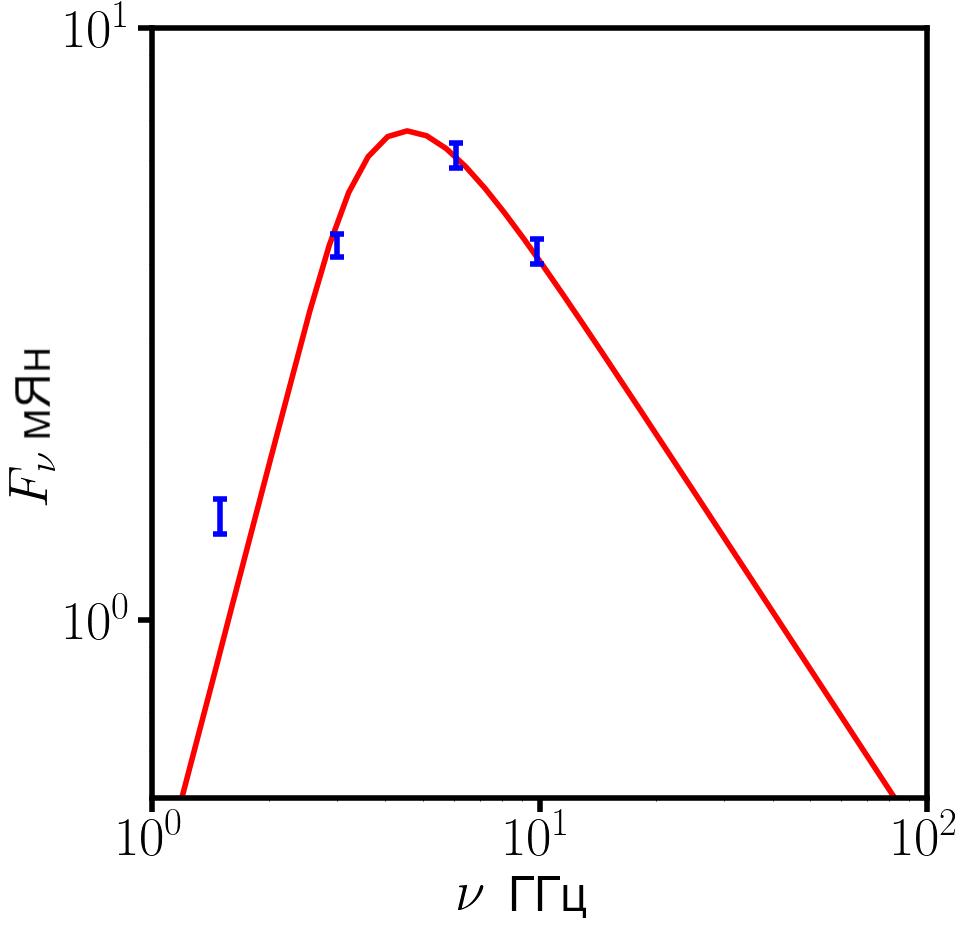
\includegraphics[width=12.5 cm]{./fig_en/synchrotron1.png} 
	\caption{Modeled spectrum of synchrotron radiation and observational data for CSS161010 at 98 day after explosion}
	\label{synchrotron1}
\end{figure}


%Пример фитирования параметров источника по наблюдательным данным приведен в функции fitTimeDependentCSS161010() в файле examples.cpp. Подберем параметры Быстрого Оптического Голубого Транзиента CSS161010 на основе наблюдений радиоизлучения, проведенных на 98, 162, 357 день после вспышки.  Расчет синхротронного излучения учитывает самопоглощение и раширение источника. Источник будем считать шаровым слоем с однородной плотностью и однороным магнитным полем, направленным перпендикулярно лучу зрения. Функцию распределения излучающих электронов возьмем на основе Particle-in-Cell расчетов для ударной волны со скоростью 0.3c,как сделано в работе \cite{BykovUniverse}. Учтена зависимость функции распределения от угла между магнитным полем и направлением распространения ударной волны.

%Подберем параметры Быстрого Оптического Голубого Транзиента CSS161010 на основе наблюдений радиоизлучения, проведенных на 98, 162, 357 день после вспышки.  Зададим сначала массивы наблюдательных точек, переведя при этом из единиц герцы и милиянские в эрги и $\text{см}^{-2} \text{c}^{-1}$
%\begin{lstlisting}[language=c++]
%const double cssx1[4] = 
%{1.5*hplank*1E9, 3.0*hplank*1E9, 6.1*hplank*1E9, %9.87*hplank*1E9};
%const double cssy1[4] =  {1.5/(hplank*1E26), 
%4.3/(hplank*1E26), 6.1/(hplank*1E26), 4.2/(hplank*1E26)};
%const double cssError1[4] = {0.1/(hplank*1E26), 
%0.2/(hplank*1E26), 0.3/(hplank*1E26), 0.2/(hplank*1E26)};
	
%const double cssx2[4] = 
%{2.94*hplank*1E9, 6.1*hplank*1E9, 9.74*hplank*1E9, %22.0*hplank*1E9};
%const double cssy2[4] = {2.9/(hplank*1E26), 
%2.3/(hplank*1E26), 1.74/(hplank*1E26), %0.56/(hplank*1E26)};
%const double cssError2[4] = {0.2/(hplank*1E26), 
%0.1/(hplank*1E26), 0.09/(hplank*1E26), %0.03/(hplank*1E26)};
	
%const double cssx3[6] = {0.33*hplank*1E9, %0.61*hplank*1E9, 
%1.5*hplank*1E9, 3.0*hplank*1E9, 6.05*hplank*1E9, %10.0*hplank*1E9};
%const double cssy3[6] = {0.375/(hplank*1E26), %0.79/(hplank*1E26), 
%0.27/(hplank*1E26),0.17/(hplank*1E26),0.07/(hplank*1E26),0.32/(hplank*1E27)};
%const double cssError3[6] = {0.375/(hplank*1E26), 0.09/(hplank*1E26),
%0.07/(hplank*1E26),0.03/(hplank*1E26),0.01/(hplank*1E26),0.8/(hplank * 1E28)};
%\end{lstlisting}

%Определим моменты времени инаблюдений и соответствующие им количества точек

%\begin{lstlisting}[language=c++]
%const int Ntimes = 3;
%double times[Ntimes] = { 99 * 24 * 3600, 162 * 24 * 3600, 357 * 24 * 3600 };
%int Nenergy[Ntimes];
%Nenergy[0] = 4;
%Nenergy[1] = 4;
%Nenergy[2] = 6;
%\end{lstlisting}
%Создадим и инициализируем необходимые массивы с наблюдательными данными
%\begin{lstlisting}[language=c++]
%double** energy = new double* [Ntimes];
%double** F = new double* [Ntimes];
%double** Error = new double* [Ntimes];
%for (int m = 0; m < Ntimes; ++m) {
%	energy[m] = new double[Nenergy[m]];
%	F[m] = new double[Nenergy[m]];
%	Error[m] = new double[Nenergy[m]];
%}

%for (int i = 0; i < Nenergy[0]; ++i) {
%	energy[0][i] = cssx1[i];
%	F[0][i] = cssy1[i];
%	Error[0][i] = cssError1[i];
%}

%for (int i = 0; i < Nenergy[1]; ++i) {
%	energy[1][i] = cssx2[i];
%	F[1][i] = cssy2[i];
%	Error[1][i] = cssError2[i];
%}

%for (int i = 0; i < Nenergy[2]; ++i) {
%	energy[2][i] = cssx3[i];
%	F[2][i] = cssy3[i];
%	Error[2][i] = cssError3[i];
%}
%\end{lstlisting}

%Зададим физические параметры источника (или их начальные приближения) - расстояние, размер, концентрацию, магнитное поле, долю толщины шара, занятую излучающим веществом, скорость расширения и магнетизацию.

%\begin{lstlisting}[language=c++]
%const double distance = 150 * 1E6 * parsec;
%double rmax = 1.3E17;
%double electronConcentration = 150;
%double B = 0.6;
%double widthFraction = 0.5;
%double v = 0.3 * speed_of_light;
%double sigma = B * B / (4 * pi * massProton * 
%electronConcentration * speed_of_light2);
%\end{lstlisting}

%Укажем для оптимизаторов количество параметров, ихи минимальные и максимальные значения и соответствие вектора параметров и физических величин. Оптимизируемыми параметрами являются - размер источника, магнетизация, доля заполнения и скорость расширения в первый момент времени, а так же показатели степени расширения со временем и изменения магнитного поля и концентрации с радиусом, то есть $\alpha, \beta, \gamma$ где эти величины определены через уравнения $R(t) = R_0 + \frac{1}{\alpha-1}\cdot V(0) \cdot t_0 \cdot ({t/t_0}^{\alpha-1}-1 )$, $B(R) = B(R_0)\cdot{R_0/R}^{\beta-1}$, $n(R) = n(R_0)\cdot{R_0/R}^{\gamma - 1}$. Единица добавлена к показателям степени для удобства численных расчетов при близости величин к нулю.
%\begin{lstlisting}[language=c++]
%const int Nparams = 8;
%double minParameters[Nparams] = { 1E16, 0.0001, 0.01, 0.1, 
%0.01 * speed_of_light, 1.1, 1.0, 1.0 };
%double maxParameters[Nparams] = { 2E17, 1, 1000, 1.0, 0.6 * 
%speed_of_light, 2.0, 3.5, 3.5 };
%double vector[Nparams] = { rmax, sigma, electronConcentration, 
%widthFraction, v, 2.0, 2.0, 3.0 };
%for (int i = 0; i < Nparams; ++i) {
%    vector[i] = vector[i] / maxParameters[i];
%}
%bool optPar[Nparams] = { true, true, true, true, true, %true, true, true };
%\end{lstlisting}

%Далее создадим источник излучения. Воспользуемся моделью расширяющейся однородной сферической оболочки, с однородным магнитным полем, перпендикулярным лучу зрения и функцией распределения электронов, зависящей от угла между направлением магнитного поля и направлением расширения оболочки. Функции распределения получены с использованием Particle-in-Cell кода Smilei \cite{Derouillat} и содержатся в директории examplesData. Методика расчетов описана в статье \cite{BykovUnirse}. Количетсво распределений, посчитанных для углов от 0 до 90 градусов равно десяти. Их можно считать из соответствующих файлов, используя метод класса MassiveParticleDistributionFactory. Так же будет добавлено продолжение мтепенного хвоста, так как PIC расчеты не пользволяют получать длинные спектры из-за большой вычислительной сложности. Так же необходимо провести масштабирование распределения, так как в PIC расчетах испольовалось уменьшенное отношение масс протонов и электронов $m_p/m_e = 100$. Имея массив распределений создадим источник, учитывающий угловую зависимость, и передим его далее источнику. учитывающему зависимость от времени.

%\begin{lstlisting}[language=c++]
%const int Ndistributions = 10;

%MassiveParticleIsotropicDistribution** angleDependentDistributions = 
%MassiveParticleDistributionFactory::readTabulatedIsotropicDistributionsAddPowerLawTail
%(massElectron, "./input/Ee", "./input/Fs", ".dat", 10, 
%DistributionInputType::GAMMA_KIN_FGAMMA, electronConcentration, 200, 20 * me_c2, 3.5);
%for (int i = 0; i < Ndistributions; ++i) {
%(dynamic_cast<MassiveParticleTabulatedIsotropicDistribution*>
%(angleDependentDistributions[i]))->rescaleDistribution(sqrt(18));
%}

%AngleDependentElectronsSphericalSource* angleDependentSource = new 
%AngleDependentElectronsSphericalSource(20, 20, 4, Ndistributions, 
%angleDependentDistributions,B,1.0,0,electronConcentration,rmax,0.5*rmax,distance);

%RadiationTimeDependentSource* source = new 
%ExpandingRemnantSource(rmax, B, electronConcentration, 0.3 * speed_of_light,
%0.5, angleDependentSource, times[0]);

%\end{lstlisting}

%Теперь создадим вычислитель синхротронного излучения и два оптимизатора параметров - первый будет работать перебором параметров по сетке, а второй - градиентным спуском. Укажем количество точек по осям для перебора, количество итераций для градиентного спуска и диапазон энергий электронов, который будет рассматривать вычислитель синхротронного излучения.

%\begin{lstlisting}[language=c++]
%int Npoints[Nparams] = { 3, 3, 3, 3, 3, 3, 3, 3 };
%int Niterations = 5;

%double Emin = me_c2;
%double Emax = 10000 * me_c2;

%SynchrotronEvaluator* synchrotronEvaluator=new %SynchrotronEvaluator(200, Emin, Emax);

%RadiationTimeOptimizer* gridEnumOptimizer = 
%new GridEnumRadiationTimeOptimizer(synchrotronEvaluator, minParameters, 
%maxParameters, Nparams, Npoints);
%RadiationTimeOptimizer* gradientOptimizer = 
%new GradientDescentRadiationTimeOptimizer(synchrotronEvaluator,minParameters, 
%maxParameters, Nparams, Niterations);
%\end{lstlisting}

%Применим созданые оптимизаторы и изменим параметры источника на найденные, соответствующие минимуму.

%\begin{lstlisting}[language=c++]

%gridEnumOptimizer->optimize(vector, optPar, energy, F, Error, Nenergy, Ntimes, times, source);

%gradientOptimizer->optimize(vector, optPar, energy, F, Error, Nenergy, Ntimes, times, source);

%source->resetParameters(vector, maxParameters);
%\end{lstlisting}

%Полученные в результате оптимизации парметры источника равны: радиус диска в начальный момент времени $R = 1.8\times10^17 \text{ см}$, магнитное поле $B = 1.6 \text{ Гс}$, концентрация электронов $n = 2.3 \text{ см}^{-3}$, доля толщины $fraction = 0.54 $, степени зависимости . Значение целевой функции $f \approx 50$. Модельный спектр излучения  с данными параметрами и наблюдательные данные изображены на рисунке \ref{synchrotronSeries}.

%\begin{figure}
%	\centering
%	%\includegraphics[width=12.5 cm]{./fig/synchrotronSeries.png} 
%	\caption{Наблюдаемый и расчетный спектр радиоизлучения объекта CSS161010 на 99, 162 и 357 дни после вспышки}
%	\label{synchrotronSeries}
%\end{figure}			% Глава 3. Формулы расчета излучения
	\addcontentsline{toc}{chapter}{\bibname}	% Добавляем список литературы в оглавление
\linespread{1}\selectfont
%\bibliography{introduction,part1,part2,part3,part4,part5}
\bibliography{part1}  
%\bibliography{part2}  
%\bibliography{part3} 
%\bibliography{part4} 
% Подключаем BibTeX-базы
		% Список литературы
	%\input{appendix}     % Приложения
	
\end{document}
